%%%% Шаблон Отчета по практике <<SPbPU-student-thesis-template>>  %%%%
%%
%%   Создан на основе глубокой переработки шаблона российских кандидатских и докторских диссертаций [1]. 
%%   
%%   Полный список различий может быть получен командами git.
%%   Лист авторов-составителей расположен в README.md файле.
%%   Подробные инструкции по использованию в [1,2].
%%   
%%   Рекомендуем установить TeX Live + TeXstudio
%%   <<Стандартная>> компиляция 2-3 РАЗА с помощью pdflatex + biber (для библиографии)     
%%  
%%%% Student thesis template <<SPbPU-student-thesis-template>> %%%%
%%
%%   Created on the basis of deep modifification of the Russian candidate and doctorate thesis template [1]. 
%%   
%%   Full list of differences can be achieved by git commands.
%%   List of template authors can be seen in the README.md file.
%%   Detailed instructions of usage, see, please in [1,2].
%%     
%%   [1] github.com/AndreyAkinshin/Russian-Phd-LaTeX-Dissertation-Template 
%%   [2] Author_guide_SPBPU-student-thesis-template.pdf
%%   
%%   It is recommended to install TeX Live + TeXstudio   
%%   Default compilation 2-3 TIMES with pdflatex + biber (for the bibliography)
%%  
\input{template_settings/ch_preamble} % лучше не редактировать / please, keep unmodified

\setcounter{docType}{2} % лучше не редактировать / please, keep unmodified

%%%% Настройки автора / Author settings
%% 
\input{my_folder/my_settings} % добавляем свои команды / update your commands


\begin{document} % начало документа
	


%%% Внесите свои данные - Input your data
%%
%%
\newcommand{\Author}{А.А.\,Гладышев} % И.О. Фамилия автора 
\newcommand{\AuthorFull}{Гладышев Александр Алексеевич} % Фамилия Имя Отчество автора
\newcommand{\AuthorFullDat}{Гладышеву Александру Алексеевичу} % Фамилия Имя Отчество автора в дательном падеже (Кому? Студенту...)
\newcommand{\AuthorFullVin}{Гладышева Александра Алексеевича} % в винительном падеже (Кого? что?  Програмиста ...)
\newcommand{\AuthorPhone}{+7-999-234-75-51} % номер телефорна автора для оперативной связи  
\newcommand{\Supervisor}{В.А.\,Пархоменко} % И. О. Фамилия научного руководителя
\newcommand{\SupervisorFull}{Владимир Андреевич Пархоменко} % Фамилия Имя Отчество научного руководителя
\newcommand{\SupervisorVin}{В.А.\,Пархоменко} % И. О. Фамилия научного руководителя  в винительном падеже (Кого? что? Руководителя ...)
\newcommand{\SupervisorJob}{должность} %
\newcommand{\SupervisorJobVin}{должность} % в винительном падеже (Кого? что?  Програмиста ...)
\newcommand{\SupervisorDegree}{степень} %
\newcommand{\SupervisorTitle}{звание} % 
%%
%%
%Руководитель, утверждающий задание
\newcommand{\Head}{В.А.\,Пархоменко} % И. О. Фамилия руководителя подразделения (руководителя ОП)
\newcommand{\HeadDegree}{Должность руководителя}% Только должность:   
%Руководитель %ОП 
%Заведующий % кафедрой
%Директор % Высшей школы
%Зам. директора
\newcommand{\HeadDep}{M} % заменить на краткую аббревиатуру подразделения или оставить пустым, если утверждает руководитель ОП

%%% Руководитель, принимающий заявление
\newcommand{\HeadAp}{И.О.\,Фамилия} % И. О. Фамилия руководителя подразделения (руководителя ОП)
\newcommand{\HeadApDegree}{Должность руководителя}% Только должность:   
%Руководитель ОП 
%Заведующий кафедрой
%Директор Высшей школы
\newcommand{\HeadApDep}{O} % заменить на краткую аббревиатуру подразделения или оставить пустым, если утверждает руководитель ОП
%%% Консультант по нормоконтролю
\newcommand{\ConsultantNorm}{И.О.\,Фамилия} % И. О. Фамилия консультанта по нормоконтролю. ТОЛЬКО из числа ППС!
\newcommand{\ConsultantNormDegree}{должность, степень} %   
%%% Первый консультант
\newcommand{\ConsultantExtraFull}{Фамилия Имя Отчетство} % Фамилия Имя Отчетство дополнительного консультанта 
\newcommand{\ConsultantExtra}{И.О.\,Фамилия} % И. О. Фамилия дополнительного консультанта 
\newcommand{\ConsultantExtraDegree}{должность, степень} % 
\newcommand{\ConsultantExtraVin}{И.О.\,Фамилию} % И. О. Фамилия дополнительного консультанта в винительном падеже (Кого? что? Руководителя ...)
\newcommand{\ConsultantExtraDegreeVin}{должность, степень} %  в винительном падеже (Кого? что? Руководителя ...)
%%% Второй консультант
\newcommand{\ConsultantExtraTwoFull}{Фамилия Имя Отчетство} % Фамилия Имя Отчетство дополнительного консультанта 
\newcommand{\ConsultantExtraTwo}{И.О.\,Фамилия} % И. О. Фамилия дополнительного консультанта 
\newcommand{\ConsultantExtraTwoDegree}{должность, степень} % 
\newcommand{\ConsultantExtraTwoVin}{И.О.\,Фамилию} % И. О. Фамилия дополнительного консультанта в винительном падеже (Кого? что? Руководителя ...)
\newcommand{\ConsultantExtraTwoDegreeVin}{должность, степень} %  в винительном падеже (Кого? что? Руководителя ...)
\newcommand{\Reviewer}{И.О.\,Фамилия} % И. О. Фамилия резензента. Обязателен только для магистров.
\newcommand{\ReviewerDegree}{должность, степень} % 
%%
%%
\renewcommand{\thesisTitle}{Тема выпускной квалификационной работы}
\newcommand{\thesisDegree}{работа бакалавра}% дипломный проект, дипломная работа, магистерская диссертация %c 2020
\newcommand{\thesisTitleEn}{Title of the thesis} %2020
\newcommand{\thesisDeadline}{дд.мм.202X}
\newcommand{\thesisStartDate}{дд.мм.202X}
\newcommand{\thesisYear}{202X}
%%
%%
\newcommand{\group}{5130903/100301} % заменить вместо N номер группы
\newcommand{\thesisSpecialtyCode}{09.03.03}% код направления подготовки
\newcommand{\thesisSpecialtyTitle}{Прикладная информатика} % наименование направления/специальности
\newcommand{\thesisOPPostfix}{YY} % последние цифры кода образовательной программы (после <<_>>)
\newcommand{\thesisOPTitle}{Наименование направленности (профиля) образовательной программы}% наименование образовательной программы
%%
%%
\newcommand{\institute}{
Институт компьютерных наук и~кибербезопасности
%Институт компьютерных наук и~технологий
%Гуманитарный институт
%Инженерно-строительный институт
%Институт биомедицинских систем и технологий
%Институт металлургии, машиностроения и транспорта
%Институт передовых производственных технологий
%Институт прикладной математики и механики
%Институт физики, нанотехнологий и телекоммуникаций
%Институт физической культуры, спорта и туризма
%Институт энергетики и транспортных систем
%Институт промышленного менеджмента, экономики и торговли
}%
%%
%%




%%% Задание ключевых слов и аннотации
%%
%%
%% Ключевых слов от 3 до 5 слов или словосочетаний в именительном падеже именительном падеже множественного числа (или в единственном числе, если нет другой формы) по правилам русского языка!!!
%%
%%
\newcommand{\keywordsRu}{Стилевое оформление сайта, управление контентом, php, MySQL, архитектура системы} % ВВЕДИТЕ ключевые слова по-русски
%%
%%
\newcommand{\keywordsEn}{Style registration, content management, php, MySQL, system architecture} % ВВЕДИТЕ ключевые слова по-английски
%%
%%
%% Реферат ОТ 1000 ДО 1500 знаков на русский или английский текст
%%
%Реферат должен содержать:
%- предмет, тему, цель ВКР;
%- метод или методологию проведения ВКР:
%- результаты ВКР:
%- область применения результатов ВКР;
%- выводы.

\newcommand{\abstractRu}{В данной работе изложена сущность подхода к созданию динамического информационного портала на основе использования открытых технологий Apache, MySQL и PHP. Даны общие понятия и классификация IT-систем такого класса. Проведен анализ систем-прототипов. Изучена технология создания указанного класса информационных систем. Разработана конкретная программная реализация динамического информационного портала на примере портала выбранной тематики...} % ВВЕДИТЕ текст аннотации по-русски
%%
%%
\newcommand{\abstractEn}{In the given work the essence of the approach to creation of a dynamic information portal on the basis of use of open technologies Apache, MySQL and PHP is stated. The general concepts and classification of IT-systems of such class are given. The analysis of systems-prototypes is lead. The technology of creation of the specified class of information systems is investigated. Concrete program realization of a dynamic information portal on an example of a portal of the chosen subjects is developed...} % ВВЕДИТЕ текст аннотации по-английски


%%% РАЗДЕЛ ДЛЯ ОФОРМЛЕНИЯ ПРАКТИКИ
%Место прохождения практики
\newcommand{\PracticeType}{Отчет о прохождении % 
	%стационарной производственной (технологической (проектно-технологической)) %
	такой-то % тип и вид ЗАМЕНИТЬ
	практики}

\newcommand{\Workplace}{СПбПУ, ИКНТ, ВШИСиСТ} % TODO Rename this variable

% Даты начала/окончания
\newcommand{\PracticeStartDate}{%
дд.мм.гггг%
%	22.06.2020
}%
\newcommand{\PracticeEndDate}{%
	дд.мм.гггг%
%	18.07.2020%
}%
%%

\newcommand{\School}{
	Высшая школа программной инженерии
%	Высшая школа интеллектуальных систем и~суперкомпьютерных~технологий 
}
\newcommand{\practiceTitle}{Тема практики}


%% ВНИМАНИЕ! Необходимо либо заменить текст аннотации (ключевых слов) на русском и английском, либо удалить там весь текст, иначе в свойства pdf-отчета по практике пойдет шаблонный текст.

%%% Не меняем дальнейшую часть - Do not modify the rest part
%%
%%
%%
%%
\ifnumequal{\value{docType}}{1}{% Если ВКР, то...
	\newcommand{\DocType}{Выпускная квалификационная работа}
	\newcommand{\pdfDocType}{\DocType~(\thesisDegree)} %задаём метаданные pdf файла
	\newcommand{\pdfTitle}{\thesisTitle}
}{% Иначе 
	\newcommand{\DocType}{\PracticeType}
	\newcommand{\pdfDocType}{\DocType} %задаём метаданные pdf файла
	\newcommand{\pdfTitle}{\practiceTitle}
}%
\newcommand{\HeadTitle}{\HeadDegree~\HeadDep}
\newcommand{\HeadApTitle}{\HeadApDegree~\HeadApDep}
\newcommand{\thesisOPCode}{\thesisSpecialtyCode\_\thesisOPPostfix}% код образовательной программы
\newcommand{\thesisSpecialtyCodeAndTitle}{\thesisSpecialtyCode~\thesisSpecialtyTitle}% Код и наименование направления/специальности
\newcommand{\thesisOPCodeAndTitle}{\thesisOPCode~\thesisOPTitle} % код и наименование образовательной программы
%%
%%
\hypersetup{%часть болка hypesetup в style
		pdftitle={\pdfTitle},    % Заголовок pdf-файла
		pdfauthor={\AuthorFull},    % Автор
		pdfsubject={\pdfDocType. Шифр и наименование направления подготовки: \thesisSpecialtyCodeAndTitle. \abstractRu},      % Тема
		pdfcreator={LaTeX, SPbPU-student-thesis-template},     % Приложение-создатель
%		pdfproducer={},  % Производитель, Производитель PDF % будет выставлена автоматически
		pdfkeywords={\keywordsRu}
}
%%
%%
%% вспомогательные команды
\newcommand{\firef}[1]{рис.\ref{#1}} %figure reference
\newcommand{\taref}[1]{табл.\ref{#1}}	%table reference
%%
%%
%% Архивный вариант задания ключевых слов, аннотации и благодарностей 
% Too hard to export data from the environment to pdf-info
% https://tex.stackexchange.com/questions/184503/collecting-contents-of-environment-and-store-them-for-later-retrieval
%заменить NewEnviron на newenvironment для распознавания команды в TexStudio
%\NewEnviron{keywordsRu}{\noindent\MakeUppercase{\BODY}}
%\NewEnviron{keywordsEn}{\noindent\MakeUppercase{\BODY}}
%\newenvironment{abstractRu}{}{}
%\newenvironment{abstractEn}{}{}
%\newenvironment{acknowledgementsRu}{\par{\normalfont \acknowledgements.}}{}
%\newenvironment{acknowledgementsEn}{\par{\normalfont \acknowledgementsENG.}}{}


%%% Переопределение именований %%% Не меняем - Do not modify
%\newcommand{\Ministry}{Минобрнауки России} 
\newcommand{\Ministry}{Министерство науки и высшего образования Российской~Федерации} %с 2020
\newcommand{\SPbPU}{Санкт-Петербургский политехнический университет Петра~Великого}
\newcommand{\SPbPUOfficialPrefix}{Федеральное государственное автономное образовательное учреждение высшего образования}
\newcommand{\SPbPUOfficialShort}{ФГАОУ~ВО~<<СПбПУ>>}
%% Пробел между И. О. не допускается.
\renewcommand{\alsoname}{см. также}
\renewcommand{\seename}{см.}
\renewcommand{\headtoname}{вх.}
\renewcommand{\ccname}{исх.}
\renewcommand{\enclname}{вкл.}
\renewcommand{\pagename}{Pages}
\renewcommand{\partname}{Часть}
\renewcommand{\abstractname}{\textbf{Аннотация}}
\newcommand{\abstractnameENG}{\textbf{Annotation}}
\newcommand{\keywords}{\textbf{Ключевые слова}}
\newcommand{\keywordsENG}{\textbf{Keywords}}
\newcommand{\acknowledgements}{\textbf{Благодарности}}
\newcommand{\acknowledgementsENG}{\textbf{Acknowledgements}}
\renewcommand{\contentsname}{Content} % 
%\renewcommand{\contentsname}{Содержание} % (ГОСТ Р 7.0.11-2011, 4)
%\renewcommand{\contentsname}{Оглавление} % (ГОСТ Р 7.0.11-2011, 4)
\renewcommand{\figurename}{Рис.} % Стиль СПбПУ
%\renewcommand{\figurename}{Рисунок} % (ГОСТ Р 7.0.11-2011, 5.3.9)
\renewcommand{\tablename}{Таблица} % (ГОСТ Р 7.0.11-2011, 5.3.10)
%\renewcommand{\indexname}{Предметный указатель}
\renewcommand{\listfigurename}{Список рисунков}
\renewcommand{\listtablename}{Список таблиц}
\renewcommand{\refname}{\fullbibtitle}
\renewcommand{\bibname}{\fullbibtitle}

\newcommand{\chapterEnTitle}{Сhapter title} % <- input the English title here (only once!) 
\newcommand{\chapterRuTitle}{Название главы}          % <- введите 
\newcommand{\sectionEnTitle}{Section title} %<- input subparagraph title in english
\newcommand{\sectionRuTitle}{Название подраздела} % <- введите название подраздела по-русски
\newcommand{\subsectionEnTitle}{Subsection title} % - input subsection title in english
\newcommand{\subsectionRuTitle}{Название параграфа} % <- введите название параграфа по-русски
\newcommand{\subsubsectionEnTitle}{Subsubsection title} % <- input subparagraph title in english
\newcommand{\subsubsectionRuTitle}{Название подпараграфа} % <- введите название подпараграфа по-русски % Заполнить сведения, 
										 % в т.ч. ключевые слова и аннотацию.

%\input{my_folder/practice}				 % Титульный лист
										 % Убираем footnotes, консультанта, если нет

\input{my_folder/contents}  	         % Оглавление


\chapter*{Введение} % * не проставляет номер
\addcontentsline{toc}{chapter}{Введение} % вносим в содержание

В современном мире информационных технологий повышение безопасности программного обеспечения является одной из ключевых проблем. С увеличением сложности программных продуктов и их широким распространением во всех сферах жизни общества, вопрос выявления и устранения уязвимостей становится особенно актуальным. 

Классические методы тестирования сталкиваются с рядом проблем, таких как невозможность предсказания всех сценариев использования ПО, сложности в обнаружении трудноуловимых ошибок и т.д. Фаззинг, как метод автоматизированного тестирования программ на наличие ошибок и уязвимостей путем подачи неожиданных или случайно сгенерированных данных на вход, показывает высокую эффективность в решении данной проблемы. Однако, несмотря на свои преимущества, фаззинг сталкивается с рядом сложностей, таких как выбор оптимальных стратегий генерации входных данных и анализ большого объема результатов тестирования.
\par

\textbf{Актуальность} применения фаззинга определяется постоянно растущими требованиями к безопасности программного обеспечения и необходимостью эффективного и своевременного обнаружения потенциальных уязвимостей. Методы фаззинга, и в частности инструменты вроде AFL++, предлагают возможность автоматизации процесса поиска ошибок, что значительно повышает шансы на их обнаружение до того, как они будут эксплуатированы пользователями. Важность фаззинга усиливается в контексте непрерывно возрастающего числа угроз информационной безопасности и роста сложности программных систем, что делает традиционные методы тестирования недостаточно эффективными.
\par

\textbf{Целью} данной работы является исследование и анализ методов фаззинга, с акцентом на использование инструмента AFL++ для выявления ошибок в программном обеспечении. %уязвимостей - это в курсе Инфобеза будет

 В рамках работы планируется детально изучить теоретические основы фаззинга, его внутреннее устройство и алгоритмы, а также провести практическое тестирование с использованием fuzz-goat~\cite{???} для демонстрации возможностей и эффективности метода. Особое внимание будет уделено анализу результатов фаззинга, выявлению и классификации обнаруженных уязвимостей, а также оценке возможностей AFL++ как инструмента для улучшения безопасности программного обеспечения.
\par
В рамках достижения поставленной цели работы определены следующие \textbf{задачи}:
\begin{enumerate}
	\item Изучение теоретических аспектов фаззинга как методики обнаружения ошибок в программном обеспечении, включая историческое развитие, основные подходы и классификацию фаззеров.
	\item Анализ внутреннего устройства и алгоритмов фаззинга, освещение принципов генерации входных данных и механизмов обнаружения ошибок.
	\item Освещение особенностей и возможностей AFL++, включая сравнение с другими инструментами фаззинга и детальное рассмотрение его функциональности.
	\item Проведение практического фаззинга на примере fuzz-goat с использованием AFL++.
	\item Выявление и анализ обнаруженных уязвимостей в ходе фаззинга fuzz-goat.
	\item Оценка эффективности AFL++ и фаззинга в целом как инструментов повышения безопасности программного обеспечения, формулирование выводов о преимуществах и ограничениях методики.
\end{enumerate}

%% Вспомогательные команды - Additional commands
%\newpage % принудительное начало с новой страницы, использовать только в конце раздела
%\clearpage % осуществляется пакетом <<placeins>> в пределах секций
%\newpage\leavevmode\thispagestyle{empty}\newpage % 100 % начало новой строки	    	 % Введение

%% Начало основной части
\chapter{Фаззинг, как методика обнаружения уязвимостей в ПО} \label{ch1}

% не рекомендуется использовать отдельную section <<введение>> после лета 2020 года
%\section{Введение. Сложносоставное название первого параграфа первой главы для~демонстрации переноса слов в содержании} \label{ch1:intro}

Фаззинг-тестирование - это тип тестирования безопасности, который позволяет обнаружить ошибки кодирования и лазейки в программном обеспечении, операционных системах или сетях. Фаззинг включает в себя ввод огромного количества случайных данных в тестируемое программное обеспечение, чтобы заставить его дать сбой. Одним из ключевых преимуществ фаззинга является его способность эффективно сканировать программное обеспечение на предмет ошибок обработки данных, таких как переполнение буфера, уязвимости для SQL-инъекций, кросс-сайтового скриптинга и других видов уязвимостей, которые могут быть эксплуатированы злоумышленниками. 
\par
Фаззинг выполняется с помощью фаззера - программы, которая автоматически вводит псевдослучайные данные в программу и обнаруживает ошибки. Фаззинг-тестирование обычно выполняется автоматически. Оно обнаруживает наиболее серьезные ошибки или дефекты безопасности и является экономически эффективным методом тестирования. Фаззинг также является одним из самых распространенных методов, используемых хакерами для обнаружения уязвимостей системы [1].


\section{Классификация фаззеров} \label{ch1:sec1}


%\subsection{Название первого подпараграфа первого параграфа первой главы для~демонстрации переноса слов в содержании} % ~ нужен, чтобы избавиться от висячего предлога (союза) в конце строки

По методу генерации новых входных значений фаззеры подразделяются на:
\begin{itemize}
	\item Mutation-Based Fuzzers: Это один из типов фаззинга, при котором фаззер имеет некоторые знания о входном формате тестируемой программы: на основе существующих выборок данных инструменты фаззинга на основе мутаций генерируют новые варианты (мутанты), которые он использует для фаззинга. Прим.: AFL++.
	\item Generation-Based Fuzzers: Фаззер генерирует входные данные с нуля. Например, использует входную модель, предоставленную пользователем, для генерации новых входных данных. Прим.: Peach Fuzzer [1].
\end{itemize}

По цели фаззинга:
\begin{itemize}
	\item Protocol-based Fuzzers. Фокусируются на тестировании безопасности сетевых протоколов и программ, обрабатывающих конкретные файловые форматы (изображения, архивы и документы и другое) Прим.: Boofuzz.
	\item Library and Framework Fuzzers. Предназначаются для тестирования функций из готовых библиотек и пакетов. Прим.: LibFuzzer, Jazzer.
	\item Binary Fuzzers. Осуществляют проверку безопасности исполняемого бинарного кода. Прим.: AFL++ (QEMU mode).
	\item API Fuzzers. Предназначаются для тестирования безопасности веб-сервисов и API. Прим.: Restler [6]. 
\end{itemize}



%Одиночные формулы оформляют в окружении \texttt{equation}, например, как указано в следующей одиночной нумерованной формуле:
%
%
%\begin{equation}% лучше не оставлять пропущенную строку (\par) перед окружениями для избежания лишних отсупов в pdf
%\label{eq:Pi-ch1} % eq - equations, далее название, ch поставлено для избежания дублирования
%\pi \approx 3,141.
%\end{equation}
%%
%%
%\begin{figure}[ht!] 
%	\center
%	\includegraphics [scale=0.27] {my_folder/images//spbpu_hydrotower}
%	\caption{Вид на гидробашню СПбПУ \cite{spbpu-gallery}} 
%	\label{fig:spbpu_hydrotower}  
%\end{figure}
%
%
%\begin{table} [htbp]% Пример оформления таблицы
%	\centering\small
%	\caption{Представление данных для сквозного примера по ВКР \cite{Peskov2004}}%
%	\label{tab:ToyCompare}		
%		\begin{tabular}{|l|l|l|l|l|l|}
%			\hline
%			$G$&$m_1$&$m_2$&$m_3$&$m_4$&$K$\\
%			\hline
%			$g_1$&0&1&1&0&1\\ \hline
%			$g_2$&1&2&0&1&1\\ \hline
%			$g_3$&0&1&0&1&1\\ \hline
%			$g_4$&1&2&1&0&2\\ \hline
%			$g_5$&1&1&0&1&2\\ \hline
%			$g_6$&1&1&1&2&2\\ \hline		
%		\end{tabular}	
%	\normalsize% возвращаем шрифт к нормальному
%\end{table}


% \firef{} от figure reference
% \taref{} от table reference
% \eqref{} от equation reference

%На \firef{fig:spbpu_hydrotower} изображена гидробашня СПбПУ, а в \taref{tab:ToyCompare} приведены данные, на примере которых коротко и наглядно будет изложена суть ВКР.


\section{Недостатки fuzzing-тестирования} \label{ch1:sec2} 
Несмотря на очевидные преимущества, фаззинг также имеет недостатки:
\begin{itemize}
	\item Само по себе fuzzing тестирование не может дать полную картину общей угрозы безопасности или ошибок.
	\item Fuzzing тестирование менее эффективно для борьбы с угрозами безопасности, которые не вызывают сбоев программы, например, с некоторыми вирусами, червями, троянами и т. д.
	\item Fuzzing тестирование может обнаружить только простые неисправности или угрозы.
	\item Для эффективной работы потребуется значительное время [7].
\end{itemize}
\par
 Тем не менее, фаззинг остается одним из самых мощных инструментов в арсенале специалистов по кибербезопасности для обнаружения и устранения уязвимостей в программном обеспечении. Применение этой методики позволяет не только улучшить качество разрабатываемых программ, но и значительно повысить уровень защиты информационных систем от внешних атак.
 
%Формулы могут быть размещены в несколько строк. Чтобы выставить номер формулы напротив средней строки, используйте окружение \verb|multlined| из пакета \verb|mathtools| следующим образом \cite{Ganter1999}:
%%
%\begin{equation} 
%\label{eq:fConcept-order-ch1}
%\begin{multlined}
%(A_1,B_1)\leq (A_2,B_2)\; \Leftrightarrow \\  \Leftrightarrow\; A_1\subseteq A_2\; \Leftrightarrow \\ \Leftrightarrow\; B_2\subseteq B_1. 
%\end{multlined}
%\end{equation}
%
%
%Используя команду \verb|\labelcref| из пакета \verb|cleveref|, допустимо следующим образом оформлять ссылку на несколько формул:
%(\labelcref{eq:Pi-ch1,eq:fConcept-order-ch1}).
%%
%%
%\input{my_folder/tex/fig-spbpu-whitehall-three-in-one} % пример подключения 3х иллюстрации в одном рисунке
%
%Пример ссылок \cite{Article,Book,Booklet,Conference,Inbook,Incollection,Manual,Mastersthesis,Misc,Phdthesis,Proceedings,Techreport,Unpublished,badiou:briefings}, а также ссылок с указанием страниц, на котором отображены номера страниц  \cite[с.~96]{Naidenova2017} или в виде мультицитаты на несколько источников \cites[с.~96]{Naidenova2017}[с.~46]{Ganter1999}. Часть библиографических записей носит иллюстративный характер и не имеет отношения к реальной литературе. 
%
%
%
%%\FloatBarrier % заставить рисунки и другие подвижные (float) элементы остановиться
%\texttt{}
%\section{Выводы} \label{ch1:conclusion}
%
%Текст выводов по главе \thechapter.
%
%Кроме названия параграфа <<выводы>> можно использовать (единообразно по всем главам) следующие подходы к именованию последних разделов с результатами по главам:
%\begin{itemize}
%	\item <<выводы по главе N>>, где N --- номер соответствующей главы;
%	\item <<резюме>>;
%	\item <<резюме по главе N>>, где N --- номер соответствующей главы.
%\end{itemize}
%
%Параграф с изложением выводов по главе \textit{является обязательным}.

%% Вспомогательные команды - Additional commands
%
%\page % принудительное начало с новой страницы, использовать только в конце раздела
%\clearpage % осуществляется пакетом <<placeins>> в пределах секций
%\newpage\leavevmode\thispagestyle{empty}\newpage % 100 % начало новой страницы	         	 % Глава 1
\ContinueChapterBegin % размещать главы <<подряд>> 
\chapter{Внутреннее устройство и алгоритмы фаззинг-тестирования} \label{ch2}
	
% не рекомендуется использовать отдельную section <<введение>> после лета 2020 года
%\section{Введение} \label{ch2:intro}

%Глава посвящена более подробным примерам оформления текстово-графических объектов.
%
%В параграфе \ref{ch2:title-abbr} приведены примеры оформления многострочной формулы и одиночного рисунка. Параграф \ref{ch2:sec-abbr} раскрывает правила оформления перечислений и псевдокода. В параграфе \ref{ch2:sec-very-short-title} приведены примеры оформления сложносоставных рисунков, длинных таблиц, а также теоремоподобных окружений.
Глава посвящена подробному рассмотрению внутреннего устройства и алгоритмов, лежащих в основе фаззинг-тестирования. Особое внимание уделяется классификации методов фаззинга, которые различаются по уровню доступа к информации о тестируемой программе. Это разделение играет ключевую роль в выборе стратегии тестирования и определяет эффективность обнаружения уязвимостей. В главе также описываются различные методы fuzzing-тестирования, каждый из которых имеет свои особенности и предпочтительные области применения.


\section{Базовые этапы фаззинг-тестирования} \label{ch2:title-abbr} %название по-русски

Далее приведем....~\cite{???}.
\begin{enumerate}[label=\arabic*.]
	\item \textit{Определение целевой системы}. Выбор программного обеспечения или системы, которая будет подвергнута тестированию. %ПА далее исправляем везде по аналогии
	\item Определение входных данных:??? Анализ типов данных, обрабатываемых системой в нормальных условиях работы.
	\item Генерация fuzzing данных: Создание или модификация данных для генерации нестандартных входных значений, которые будут использоваться в тестах.
	\item Проведение теста с fuzzing данными: Подача сгенерированных данных в систему и наблюдение за её реакцией.
	\item Мониторинг поведения системы: Наблюдение за системой во время тестирования для выявления аномалий, сбоев и других нештатных ситуаций.
	\item Фиксация обнаруженных дефектов: Запись всех найденных проблем и уязвимостей в журнал дефектов для дальнейшего анализа.
	\item Анализ и устранение дефектов: Оценка выявленных уязвимостей и разработка решений для их исправления, направленных на повышение безопасности и надежности тестируемой системы [8].
\end{enumerate}

\newpage
На \firef{fig:fuzzer-works-ch2} приведён принцип работы фаззера.

\begin{figure}[ht] 
	\center
	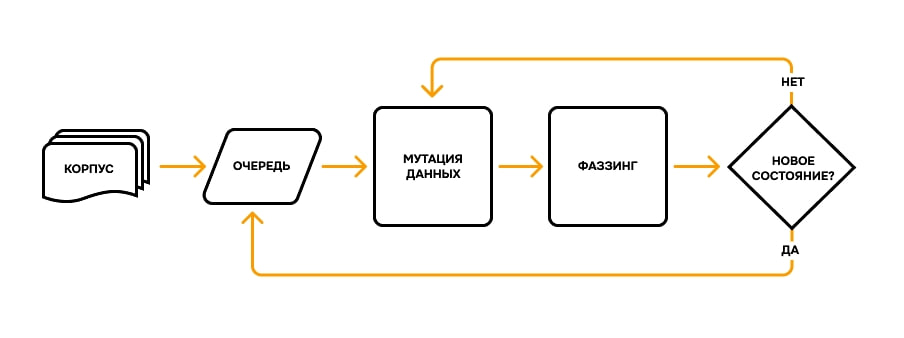
\includegraphics [scale=0.8] {my_folder/images/fuzzer_principe}
	\caption{Принцип работы фаззера} 
	\label{fig:fuzzer-works-ch2}  
\end{figure}

%%%%
%%		
%%  \input{...} commands are used only to sychronize some parts of the text with the author guide. Authors are free to type the text directly in .tex-files   
%%  \input{...} комманды используются только, чтобы синхронизировать части текта с рекомендациями авторам. Авторы  вольны вносить текст непосредственно в файл главы  
%%  
% \input{my_folder/tex/eq-Galois} % пример двух выравнивания двух формул в окружении align
%
%
%На \firef{fig:spbpu-new-bld-autumn-ch2} приведёна фотография Нового научно-исследовательского корпуса СПбПУ.
%
%	\begin{figure}[ht] 
%	\center
%	\includegraphics [scale=0.27] {my_folder/images/spbpu_new_bld_autumn}
%	\caption{Новый научно-исследовательский корпус СПбПУ \cite{spbpu-gallery}} 
%	\label{fig:spbpu-new-bld-autumn-ch2}  
%	\end{figure}
	


	
\section{Классификация методов фаззинга по уровню доступа к информации} \label{ch2:sec-abbr} %название по-русски
	Выделяют три вида фаззинга~\cite{???}: \textit{фаззинг чёрного ящика, фаззинг серого ящика и фаззинг белого ящика}, в зависимости от того, сколько информации требуется фаззеру от тестируемой программы во время исполнения. 
	
	Это разделение весьма условно, на практике, например, фаззеры белого ящика часто используют некоторые аппроксимации~\cite{???}. Термин \textit{«черный ящик»}, обычно использующийся при тестировании программного обеспечения, в случае с фаззингом обозначает аналогичное: фаззер во время своей работы не получает никакой информации от тестируемой программы, он может взаимодействовать с программой только через ввод/вывод программы. Большинство традиционных фаззеров относят к этой категории. 
	\par
	%%% ПА здесь не может быть Вашего текста:
	\textit{Фаззинг белого ящика} — противоположность чёрного. Здесь программа анализирует внутреннее устройство тестируемой программы.
	Такой фаззер использует метод, который теоретически может исследовать все пути выполнения в тестируемой программе. В отличие от фаззинга черного ящика, фаззингу белого ящика требуется информация от тестируемой программы и она используется для руководства генерацией тестов. 
	
	В частности, начиная исполнение с заданным конкретным входом, фаззер белого ящика сначала собирает символьные ограничения для всех условных операторов на пути исполнения. Следовательно, после одного исполнения такой фаззер объединяет все символьные ограничения с помощью конъюнкции для формирования ограничения пути. Затем фаззер белого ящика последовательно отрицает одно из ограничений и решает новое ограничение пути~\cite{???}. Накладные расходы на фаззинг белого ящика обычно значительно превосходят расходы на фаззинг черного ящика. Это связано с тем, что реализации динамического символьного исполнения часто используют динамические инструменты и SMT-решатели, что весьма трудоёмко. Фаззинг серого ящика — что-то среднее между первыми двумя видами. 
	\par
	\textit{Фаззер серого ящика} может получать некоторую информацию о внутренней структуре тестируемой программы и/или её исполнении. Фаззеры серого ящика полагаются на приблизительную информацию, чтобы увеличить скорость и иметь возможность тестировать программу на большем количестве входных данных [3].
	
	На \firef{fig:white-gray-black-box-ch2} представлено сравнение подходов к тестированию ПО.
	
	\begin{figure}[ht] 
		\center
		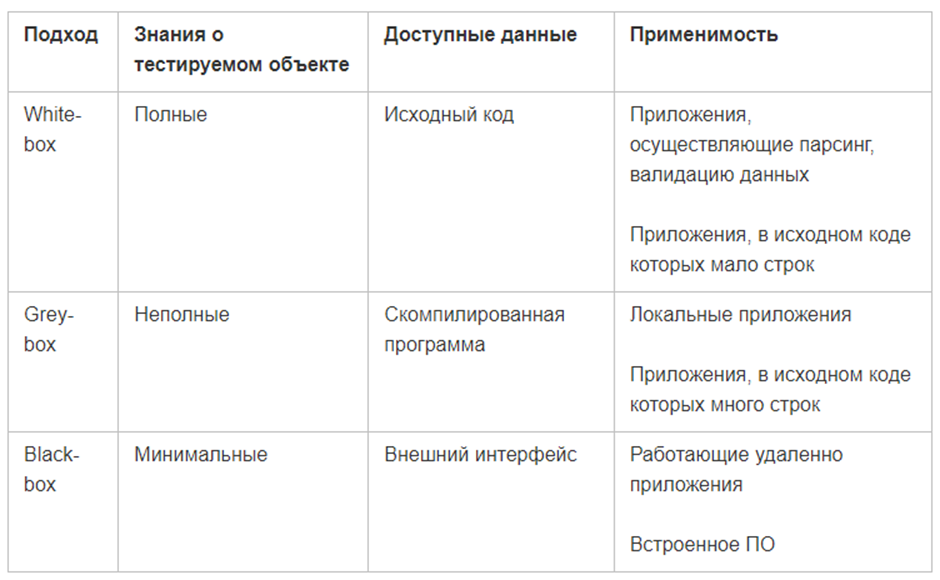
\includegraphics [scale=1] {my_folder/images/white-gray-black-box}
		\caption{Подходы к тестированию ПО [9]} 
		\label{fig:white-gray-black-box-ch2}  
	\end{figure}
	
%Название параграфа оформляется с помощью команды \verb|\section{...}|, название главы --- \verb|\chapter{...}|. 
%	
%
%\subsection{Название подпараграфа} \label{ch2:subsec-title-abbr} %название по-русски
%
%
%Название подпараграфа оформляется с помощью команды  \texttt{\textbackslash{}subsection\{...\}}.
%
%
%%\subsubsection{Название подподпараграфа} \label{ch2:subsubsec-title-abbr} %название по-русски
%	
%Использование подподпараграфов в основной части крайне не рекомендуется. В случае использования, необходимо вынести данный номер в содержание.	
%Название подпараграфа оформляется с помощью команды  \texttt{\textbackslash{}subsubsecti\-on\{...\}}.
%
%
%
%\input{my_folder/tex/enumeration} % правила использования перечислений	

	
%Оформление псевдокода необходимо осуществлять с помощью пакета \verb|algorithm2e| в окружении \verb|algorithm|. Данное окружение интерпретируется в шаблоне как рисунок. Пример оформления псевдокода алгоритма приведён на \firef{alg:AlgoFDSCALING}. 
%	
%	
%\input{my_folder/tex/pseudocode-agl-DTestsFDScaling} % пример оформления псевдокода алгоритма 	
%
%	
\section{Методы генерации данных fuzzing-тестирования} \label{ch2:sec-very-short-title} %название по-русски
\subsection{Случайное тестирование}\label{ch2:random-test}
Генерация начинается со случайных входных
данных в качестве аргументов, а затем используются некоторые дополнительные знания для получения новых входных данных. Одним
из основных представителей этой категории методов является случайное тестирование с обратной связью, которое улучшает генерацию
тестов за счёт полученной с предыдущих итераций обратной связи, которая направляет процесс создания входных данных на последующих
итерациях. 

Это позволяет снизить количество повторяющихся и/или
недопустимых входных данных, используемых для тестирования.
Инструменты для генерации тестов, использующие методы случайного тестирования, обладают преимуществами масштабируемости и простоты реализации, но используют много ресурсов на генерацию недопустимых, бесполезных (не улучшающих покрытие) входных данных ввиду случайной природы методов. Добавление обратной
связи позволяет нивелировать данный недостаток [3].%% ПА: ссылки ставят и в начале разделов, если и там есть заимствования. Здесь как будто только в последнем предложении.


\subsection{Тестирование на основе поиска}\label{ch2:search-test}
При тестировании на основе поиска задача генерации тестов решается с
помощью алгоритмов поиска, например, генетических алгоритмов. В таком случае генерация входных данных формулируется как проблема поиска, множество возможных входных значений формирует пространство решений,
а метрика, которую хочется максимизировать, например, покрытие кода, кодируется как функция приспособленности. Таким образом, поиск
будет осуществляться с помощью выбранной функции приспособленности, которая представляет из себя эвристику, оценивающую, насколько
близко текущее решение к оптимальному. Руководствуясь функцией
приспособленности, алгоритм поиска итеративно выдаёт лучшие решение до тех пор, пока либо не будет найдено оптимальное решение, либо
не будет выполнено условие остановки (например, истечение выделенного на генерацию времени) [3].

\subsection{Символьное тестирование}\label{ch2:symbol-test}
Тестирование с помощью символьного исполнения — это аналитический подход, основанный на
правилах вывода. Он использует символьные переменные как входные
данные программы и представляет значения программных переменных
как символьные выражения, а путь исполнения — выражением над символьными переменными (ограничением пути). Символьное исполнение применяется для поиска всех возможных путей исполнения программы. Данный подход способен находить пути исполнения программы, которые вызывают ошибки, даже без компиляции. Для решения
ограничений пути, как правило, применяется SMT-решатель, который
вычисляет уже конкретные значения переменных, необходимых для того, чтобы поток исполнения пошёл по данному пути. Несмотря на очевидные преимущества и силу, этот подход обычно реализуется в мелком масштабе, так как в крупных проектах наблюдается значительный рост всех возможных путей исполнения, что требует серьёзных вычислительных ресурсов. Именно по этой причине этот подход только
недавно стал применяться для генерации тестов, хотя идея символьного
исполнения появилась в 70-х годах [3].
	
%\input{my_folder/tex/eq-equation-multilined} % пример оформления одиночной формулы в несколько строк
%
%\input{my_folder/tex/fig-spbpu-sc-four-in-one} % пример подключения 4х иллюстраций в одном рисунке
%
%%\input{my_folder/tex/fig-spbpu-whitehall-three-in-one} % пример подключения 3х иллюстрации в одном рисунке
%%
%%\input{my_folder/tex/fig-spbpu-main-bld-two-in-one} % пример подключения 2х иллюстраций в одном рисунке
%
%\input{my_folder/tex/tab-more-than-one-page} % пример подключения таблицы на несколько страциц
%
%
%\begin{table} [htbp]% Пример оформления таблицы
%	\centering\small
%	\caption{Пример представления данных для сквозного примера по ВКР \cite{Peskov2004}}%
%	\label{tab:ToyCompare}		
%		\begin{tabular}{|l|l|l|l|l|l|}
%			\hline
%			$G$&$m_1$&$m_2$&$m_3$&$m_4$&$K$\\
%			\hline
%			$g_1$&0&1&1&0&1\\ \hline
%			$g_2$&1&2&0&1&1\\ \hline
%			$g_3$&0&1&0&1&1\\ \hline
%			$g_4$&1&2&1&0&2\\ \hline
%			$g_5$&1&1&0&1&2\\ \hline
%			$g_6$&1&1&1&2&2\\ \hline		
%		\end{tabular}
%%	\caption*{\raggedright\hspace*{2.5em} Составлено (или/и рассчитано) по \cite{Peskov2004}} %Если проведена авторская обработка или расчеты по какому-либо источнику	
%	\normalsize% возвращаем шрифт к нормальному
%\end{table}
%
%
%
%%% please, before using, read the author guide carefully
%
%\input{my_folder/tex/tab-toy-context-minipage} % пример подключения minipage
%
%\input{my_folder/tex/fig-spbpu-new-bld-autumn-minipage} % пример подключения minipage
%
%
%
%
%\input{my_folder/tex/rules-theorem-like-expressions} 
%
%По аналогии с нумерацией формул, рисунков и таблиц нумеруются и иные текстово-графические объекты, то есть включаем в нумерацию номер главы, например: теорема 3.1. для первой теоремы третьей главы монографии. Команды \LaTeX{} выставляют нумерацию и форматирование автоматически. Полный перечень команд для подготовки текстово-графических и иных объектов находится в подробных методических рекомендациях \cite{spbpu-bci-template-author-guide}. 
%
%
%\input{my_folder/tex/rules-list-of-environments} % список некоторых окружений
%
%
%\input{my_folder/tex/theorem-example} %пример оформления теоремы
%
%
%\input{my_folder/tex/definition-example} %пример оформления определения
%
%
%Вместо теоремо-подобных окружений для вставки небольших текстово-графических объектов иногда используются команды. Типичным примером такого подхода является команда \verb|\footnote{text}|\footnote{Внимание! Команда вставляется непосредственно после слова, куда вставляется сноска (без пробела). Лишние пробелы также не указываются внутри команды перед и после фигурных скобок.}, где в аргументе \verb|text| указывают текст \textit{подстрочной ссылки (сноски)}.В них \textit{нельзя добавлять веб-ссылки или цитировать литературу}. Для этих целей используется список литературы. Нумерация сносок сквозная по ВКР без точки на конце выставляется в шаблоне автоматически, однако в каждом приложении к ВКР нумерация, зависящая от номера приложения, выставляется префикс <<П>>, например <<П1.1>> --- первая сноска первого приложения. 
%
%
%
%
%%\FloatBarrier % заставить рисунки и другие подвижные (float) элементы остановиться
%
%
%\section{Выводы} \label{ch2:conclusion}
%
%Текст заключения ко второй главе. Пример ссылок \cite{Article,Book,Booklet,Conference,Inbook,Incollection,Manual,Mastersthesis,Misc,Phdthesis,Proceedings,Techreport,Unpublished,badiou:briefings}, а также ссылок с указанием страниц, на котором отображены те или иные текстово-графические объекты  \cite[с.~96]{Naidenova2017} или в виде мультицитаты на несколько источников \cites[с.~96]{Naidenova2017}[с.~46]{Ganter1999}. Часть библиографических записей носит иллюстративный характер и не имеет отношения к реальной литературе. 
%
%Короткое имя каждого библиографического источника содержится в специальном файле \verb|my_biblio.bib|, расположенном в папке \verb|my_folder|. Там же находятся исходные данные, которые с помощью программы \texttt{Biber} и стилевого файла \texttt{Biblatex-GOST} \cite{ctan-biblatex-gost} приведены в списке использованных источников согласно ГОСТ 7.0.5-2008.
%Многообразные реальные примеры исходных библиографических данных можно посмотреть по ссылке \cite{ctan-biblatex-gost-examples}.
%
%Как правило, ВКР должна состоять из четырех глав. Оставшиеся главы можно создать по образцу первых двух и подключить с помощью команды \verb|\input| к исходному коду ВКР. Далее в приложении \ref{appendix-MikTeX-TexStudio} приведены краткие инструкции запуска исходного кода ВКР \cite{latex-miktex,latex-texstudio}.
%
%В приложении \ref{appendix-extra-examples} приведено подключение некоторых текстово-графических объектов. Они оформляются по приведенным ранее правилам. В качестве номера структурного элемента вместо номера главы используется <<П>> с номером главы. Текстово-графические объекты из приложений не учитываются в реферате.
%
%
%
%%% Вспомогательные команды - Additional commands
%%
%%\newpage % принудительное начало с новой страницы, использовать только в конце раздела
%%\clearpage % осуществляется пакетом <<placeins>> в пределах секций
%\newpage\leavevmode\thispagestyle{empty}\newpage % 100 % начало новой страницы	         	 % Глава 2
\chapter{Инструмент фаззинг-тестирования AFL++} \label{ch3}

% не рекомендуется использовать отдельную section <<введение>> после лета 2020 года
%\section{Введение} \label{ch3:intro}

\textit{AFL++} - это улучшенная версия популярного инструмента фаззинга AFL (American Fuzzy Lop), разработанная сообществом для повышения его эффективности и функциональности. \textit{AFL} — это ориентированный на поиск ошибок инструмент анализа ПО, который использует обширный список типов инструментации кода для получения информации о покрытии и множество генетических алгоритмов мутации для автоматического обнаружения различных тестовых примеров, которые вызывают новые внутренние состояния в бинарном коде ПО.

 Фаззер AFL поддерживает инструментацию, реализующуюся на этапе компиляции из исходного кода с помощью оберток afl-gcc/afl-g++. afl-gcc/afl-g++ подменяет вызываемую команду на обертку, переписывающую ассемблерный код, сгенерированный компилятором. Для фаззинга уже скомпилированных бинарных файлов используется qemu mode — это патч к QEMU, эмулирующий запуск одного процесса и реализующий требуемую для анализа инструментацию кода [8].
\par
AFL является одним из самых известных фаззеров серого ящика, он поддерживает фаззинг программ, написанных на C, C++ и Objective C, скомпилированных с помощью и GCC, и CLang, но его часто расширяют и портируют.
\par
AFL требует от пользователя предоставить пример команды, запускающей тестируемое приложение, и хотя бы один небольшой пример входных данных. Входные данные могут быть переданы в тестируемую программу либо через стандартный ввод, либо в виде входного файла, указанного в командной строке процесса. Чтобы максимизировать производительность фаззинга, American fuzzy lop ожидает, что тестируемая программа будет скомпилирована с помощью служебной программы, которая оснащает (инструментирует) код вспомогательными функциями, которые отслеживают поток управления.

\section{Инструментирование} \label{ch3:sec1}
Инструментирование – это процесс внедрения дополнительного кода или инструкций в исходный код программы с целью сбора информации о её выполнении.
Это позволяет фаззеру:
\begin{itemize}
	\item Отслеживать, какие части кода выполняются (покрытие кода).
	\item Определять, какие новые ветви кода (пути выполнения) были исследованы благодаря новым или мутированным входным данным.
	\item Собирать статистику о выполнении для последующего анализа.
\end{itemize}
\par
AFL представляет собой фаззер серого ящика , то есть он внедряет инструменты для измерения покрытия кода в целевую программу во время компиляции и использует метрику покрытия для управления генерацией новых входных данных.
В случаях, когда это невозможно, также поддерживается тестирование «черного ящика» [2].

\section{Измерение покрытия} \label{ch3:sec2}
AFL подсчитывает количество раз, которое данное выполнение целевой программы проходит через каждое ребро в графе управления потоком целевой программы. Ребро в графе управления потоком (control-flow graph, CFG) программы представляет собой переход между двумя узлами (которые представляют собой отдельные блоки инструкций)~\cite{???}. 
\par
AFL поддерживает глобальный набор пар (словарь) которые были произведены любым выполнением до этого момента. Входные данные считаются "интересными" и добавляются в очередь, если они производят пару, которой ещё нет в словаре.
\par
Инструментарий, внедряемый в скомпилированные программы, фиксирует покрытие ветвей (рёбер), а также подсчеты срабатываний условных переходов. Точки ветвления в контексте программирования — это места в коде, где происходит условный переход, который может изменить путь выполнения программы. Например, это могут быть операторы if, switch, циклы, или даже вызовы функций — все, что может привести к изменению последовательности исполняемых инструкций [4]. 
\par
Код, вставляемый в точках ветвления, по существу включает следующее:

\begin{algorithm}
	\SetAlgoLined 
	\DontPrintSemicolon 
	
	\BlankLine
	$cur\_location \gets \langle COMPILE\_TIME\_RANDOM \rangle$\;
	\BlankLine
	\ForEach{$prev\_location$}{
		$shared\_mem[cur\_location \oplus prev\_location]++$\;
		$prev\_location \gets cur\_location \gg 1$\;
	}
	\caption{Код, измеряющий покрытие, внедряемый в точки ветвления~\cite{???}}
	\label{alg:AlgoFDSCALING}
\end{algorithm}

\textbf{cur\textunderscore location}~---это переменная, которая используется как идентификатор текущего места в коде, где выполняется операция инструментирования. Значение cur\textunderscore location генерируется случайно на этапе компиляции и уникально для каждой точки ветвления. Оно используется для того, чтобы отслеживать, была ли достигнута эта точка ветвления при выполнении программы.

\textbf{shared\textunderscore mem}:???
shared\textunderscore mem — это массив, который используется как словарь покрытия для отслеживания, какие точки ветвления (и переходы между ними) были выполнены во время исполнения программы. Ключем является xor (prev\textunderscore location, cur\textunderscore location), а значением счетчик попаданий для данного кортежа (перехода). Каждый раз, когда исполнение программы проходит через этот переход, счетчик увеличивается

\textbf{prev\textunderscore location}
помогает отслеживать предыдущее состояние исполнения программы и выявлять изменения в путях исполнения при каждой новой итерации фаззинга.

\par
Размер словаря выбран таким образом, чтобы коллизии возникали редко для почти всех предполагаемых целей. Коллизии могут возникать, например, когда несколько различных входных данных приводят к одной и той же точке ветвления (branch) в программе или к одному и тому же состоянию программы.
На \firef{fig:coverage-measuring-ch3} представлена зависимость количества коллизий от количества ветвлений.

\begin{figure}[ht] 
	\center
	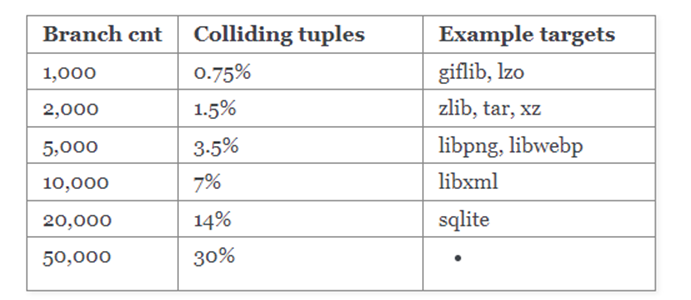
\includegraphics [scale=1] {my_folder/images/coverage_measuring}
	\caption{Распределение количества коллизий кортежей при различном количестве ветвлений для разных целей фаззинга~\cite{???}} 
	\label{fig:coverage-measuring-ch3}  
\end{figure}

В то же время размер словаря достаточно мал, чтобы анализ словаря занимал всего лишь несколько микросекунд и чтобы словарь легко помещался в кэш второго уровня (L2 cache) [4].
\par
Такая КАКАЯконкретно??? форма покрытия предоставляет значительно более глубокое представление о пути выполнения программы, в частности, она тривиально различает следующие трассы исполнения:
\par
A -> B -> C -> D -> E (кортежи: AB, BC, CD, DE) и 
\par
A -> B -> D -> C -> E (кортежи: AB, BD, DC, CE)

\section{Обнаружение нового поведения} \label{ch3:sec3}
Фаззер поддерживает глобальный словарь кортежей, замеченных в предыдущих исполнениях, эти данные можно быстро сравнить с отдельными трассами и обновить~\cite{???}.
\par
Когда измененный вход генерирует трассировку выполнения, которая содержит новые кортежи, соответствующий входной файл будет сохранен и направлен для дополнительной обработки позже. Входы, которые не инициируют новые переходы состояний локального масштаба во время отслеживания выполнения (например, не генерируют новые кортежи), будут отброшены, даже если их общий поток управления уникален.
\par
В дополнение к обнаружению новых кортежей фаззер также учитывает приблизительное количество кортежей. Они разделены на несколько частей~\cite{???}:
1, 2, 3, 4-7, 8-15, 16-31, 32-127, 128+.
\par
Эта упрощенная классификация помогает фаззеру быстро определить "интересные" изменения в потоке управления программы без необходимости в точном подсчете каждого выполнения. Вместо того, чтобы отслеживать каждое выполнение отдельно, фаззер смотрит на общую картину и обнаруживает изменения, которые выходят за пределы ожидаемых или типичных паттернов выполнения программы.

\section{Изменение очереди ввода} \label{ch3:sec4}
Тестовые случаи мутации, которые генерируют новые переходы состояний в программе, добавляются во входную очередь и служат отправной точкой для будущих циклов фаззинга. Они дополняют, но не могут автоматически заменить существующие открытия.
В отличие от более жадных генетических алгоритмов, этот подход позволяет инструменту постепенно исследовать различные непересекающиеся и, возможно, взаимно несовместимые функции базового формата данных, как показано на \firef{fig:test-generation-ch3} [4].

На \firef{fig:coverage-measuring-ch3} представлена зависимость количества коллизий от количества ветвлений.

\begin{figure}[ht] 
	\center
	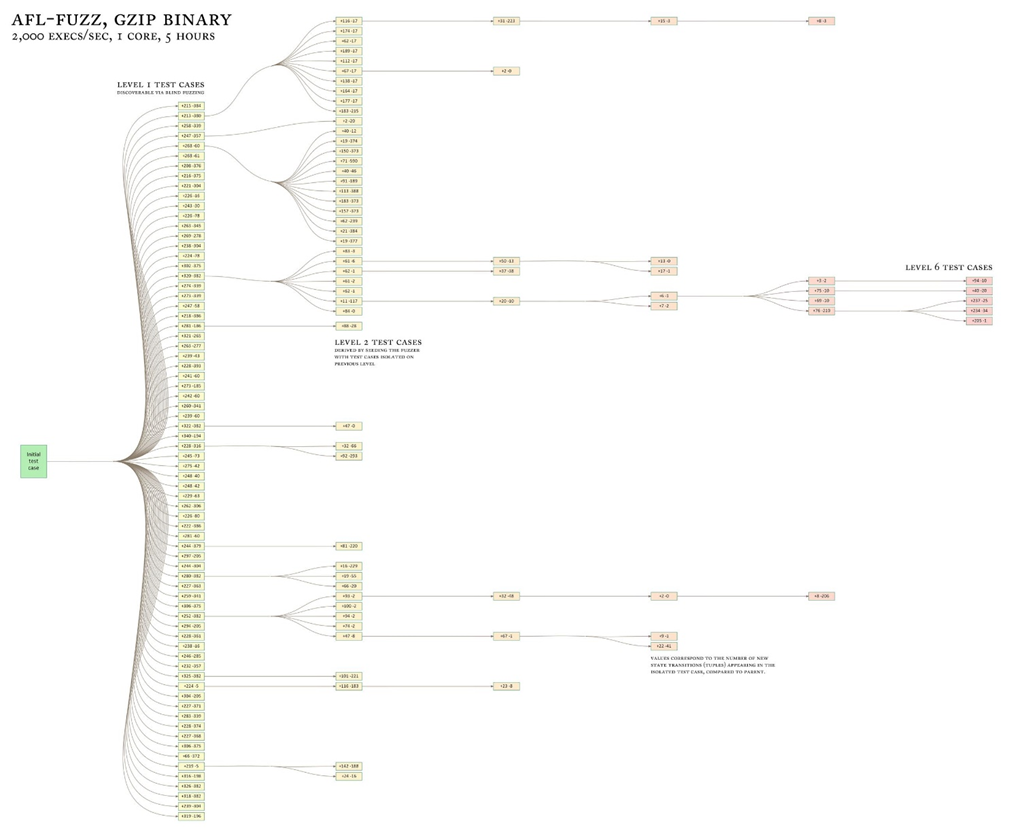
\includegraphics [scale=1] {my_folder/images/test_gen}
	\caption{Визуализация дерева тестирования AFL-Fuzz~\cite{???}} 
	\label{fig:test-generation-ch3}  
\end{figure}
\par
В общем, AFL поддерживает очередь, и каждый раз, когда файл берется из этой очереди, в нее вносится множество мутаций, и проверяется, не обнаружит ли новые пути после операции.

\section{Отбраковка корпуса} \label{ch3:sec5}
Корпус (corpus) - это коллекция тестовых данных или файлов, которые используются для проведения тестирования программы или системы~\cite{???}. Корпус включает в себя как исходные тестовые данные, так и те, которые были сгенерированы или изменены в ходе тестирования.
\par
Подход к пошаговому исследованию состояний, описанный выше, означает, что некоторые тестовые случаи, синтезированные позднее, могут иметь покрытие ветвей, которое является строгим надмножеством покрытия, предоставленного их предками. Чтобы оптимизировать процесс фаззинга, AFL периодически переоценивает очередь, используя быстрый алгоритм, который выбирает меньшее подмножество тестовых примеров, которые по-прежнему охватывают каждый кортеж, виденный на данный момент, и характеристики которых делают их особенно благоприятными для инструмента.
\par 
Сгенерированный корпус "предпочтительных" записей обычно в 5-10 раз меньше, чем исходный набор данных. Непредпочтительные записи не удаляются, но они пропускаются с различными вероятностями при обнаружении в очереди:

\begin{itemize}
	\item Если в очереди есть новые, еще не прошедшие фаззинг, предпочтительные записи, 99\% непредпочтительных записей будут пропущены, чтобы достичь предпочтительных.
	\item Если нет новых предпочтительных записей:
	\begin{itemize}
		\item Если текущая непредпочтительная запись уже прошла через фаззинг, она будет пропущена в 95\% случаев.
		\item Если она еще не прошла ни одного фаззинга, вероятность пропуска уменьшается до 75\%.
	\end{itemize}
\end{itemize}

\par
Это обеспечивает разумный баланс между скоростью цикла очереди и разнообразием тестовых случаев [4].

\section{Стратегии фаззинга, предоставляемые AFL++} \label{ch3:sec6}

Для генерации новых входных данных AFL применяет различные мутации к существующим данным. Эти мутации в основном нечувствительны к формату входных данных целевой программы; они обычно обрабатывают входные данные как простой массив бинарных данных.

Сначала AFL применяет детерминированную последовательность мутаций к каждому входному файлу. Они применяются в различных местах входных данных и включают:
\begin{itemize}
	\item Инвертирование (т.е. отрицание или инвертирование) от 1 до 32 бит.
	\item Инкрементирование и декрементирование 8-, 16- и 32-битных целых чисел в кодировках как little-endian, так и big-endian.
	\item Перезапись частей входных данных "примерно двумя десятками 'интересных' значений", включая ноль, максимальные и минимальные знаковые и беззнаковые целые различной ширины, также в кодировках little- и big-endian.
	\item Замена частей входных данных данными, взятыми из "словаря" пользовательских или автоматически обнаруженных токенов (например, магические байты или ключевые слова в текстовом формате).
\end{itemize}

После применения всех доступных детерминированных мутаций AFL переходит к стадии "havoc", на которой подряд применяются от 2 до 128 мутаций. Эти мутации включают описанные выше детерминированные мутации, а также:
\begin{itemize}
	\item Перезапись байтов случайными значениями.
	\item Операции над многобайтовыми "блоками":
	\begin{itemize}
		\item Удаление блоков.
		\item Дублирование блоков.
		\item Установка каждого байта в блоке в одно значение.
	\end{itemize}
\end{itemize}

Если AFL проходит через всю очередь, не генерируя ни одного входа, который достигает нового покрытия кода, он начинает "склеивание". Склеивание берет два входа из очереди, обрезает их в произвольных позициях, соединяет их вместе и применяет к результату стадию "havoc"  [2].

\subsection{Стратегия фаззинга: Bit flips} \label{ch2:bit-flips}
Первая и наиболее элементарная стратегия, используемая afl включает в себя выполнение последовательных, упорядоченных переворотов битов. Переход всегда составляет один бит; количество бит, переворачиваемых подряд, варьируется от одного до четырех. Для большого и разнообразного массива входных файлов наблюдаемые результаты следующие~\cite{???}:

\begin{itemize}
	\item Переключение одного бита: ~ 70 новых путей на миллион сгенерированных входных данных
	\item Переключение двух битов подряд: ~ 20 дополнительных путей на миллион сгенерированных входных данных
	\item Переключение четырех битов подряд: ~ 10 дополнительных путей на миллион входных данных [5].
\end{itemize}

\begin{figure}[ht]
	\begin{lstlisting}[language=C]
		#define FLIP_BIT(_ar, _b) do { 
			u8 *_arf = (u8 *)(_ar);      
			u32 _bf = (_b);              
			_arf[(_bf) >> 3] ^= (128 >> ((_bf) & 7)); 
		} while (0)
	\end{lstlisting}
	\caption{Реализация алгоритма bit flip в AFL++~\cite{???}}\label{fig:flip-bit}
\end{figure}

Этот макрос переворачивает конкретный бит в массиве. Он использует \textunderscore ar для указания на массив, а \textunderscore b для указания на бит, который нужно перевернуть. Переворот осуществляется путём применения операции XOR к соответствующему байту и биту в этом байте.

\subsection{Стратегия фаззинга: Byte flips} \label{ch2:byte-flips}
Естественное продолжение подхода пошагового переворота битов, этот метод основан на битовых переворотах шириной 8, 16 или 32 бита с постоянным переходом на один байт. Эта стратегия обнаруживает около ~ 30 дополнительных путей на миллион входных данных, в дополнение к тому, что могло бы быть запущено при более коротких переключениях битов. В AFL++ byte flips реализован аналогично bit flips [5].

\subsection{Стратегия фаззинга: Simple arithmetics} \label{ch2:simple-arithmetics}
Этап состоит из трех отдельных операций~\cite{???}. Сначала фаззер пытается выполнить вычитание и сложение для отдельных байтов. Второй проход включает просмотр 16-битных значений с использованием обоих порядковых значений, но увеличивая или уменьшая их только в том случае, если операция также повлияла бы на самый старший байт (в противном случае операция просто дублировала бы результаты 8-битного прохода). Заключительный этап следует той же логике, но для 32-битных целых чисел [5].

Рассмотрим часть кода, отвечающую за мутацию 8-ми битных значений:

\begin{figure}[ht]
	\begin{lstlisting}[language=C]
	for (i = 0; i < (u32)len; ++i) {
	u8 orig = out_buf[i];
	if (!skip_eff_map[i]) continue;
	for (j = 1; j <= ARITH_MAX; ++j) {
		u8 r = orig ^ (orig + j);
		if (!could_be_bitflip(r)) {
			out_buf[i] = orig + j;
			if (common_fuzz_stuff(afl, out_buf, len)) { goto abandon_entry; }
		}
		out_buf[i] = orig - j;
		if (!could_be_bitflip(r)) {
			if (common_fuzz_stuff(afl, out_buf, len)) { goto abandon_entry; }
		}
		out_buf[i] = orig;
	}
}
	\end{lstlisting}
	\caption{Реализация алгоритма simple arithmetic в AFL++~\cite{???}}\label{fig:simple-arithmetic}
\end{figure}
\newpage
Этот код проходит через каждый байт входных данных, пытаясь прибавить и вычесть к нему значения от 1 до ARITH\textunderscore MAX. Мутация применяется только если результат операции не может быть достигнут с помощью простого битфлипа, что позволяет сосредоточиться на более сложных и интересных случаях. После каждой мутации вызывается функция common\textunderscore fuzz\textunderscore stuff, которая запускает тестируемое приложение с мутированными данными и проверяет результаты на наличие ошибок.


Эта стратегия помогает обнаруживать ошибки, связанные с некорректной обработкой числовых значений, такие как переполнения или неправильные граничные условия, что делает её важной частью процесса фаззинга.

%\FloatBarrier % заставить рисунки и другие подвижные (float) элементы остановиться

\subsection{Стратегия фаззинга: Known integers} \label{ch2:known-ints}
AFL полагается на жестко запрограммированный набор целых чисел, выбранных из-за их явно повышенной вероятности запуска граничных условий в типичном коде (например, -1, 256, 1024, MAX\textunderscore INT-1, MAX\textunderscore INT)~\cite{???}. Фаззер использует переход на один байт, чтобы последовательно перезаписать существующие данные во входном файле одним из примерно двух десятков "интересных" значений, используя оба порядковых номера (записи имеют ширину 8, 16 и 32 бита).


Эффективность на этом этапе составляет от 2 до 5 дополнительных путей на миллион попыток [5].

\subsection{Стратегия фаззинга: Stacked tweaks} \label{ch2:stacked-tweaks}
Когда детерминированные стратегии исчерпаны для конкретного входного файла, фаззер продолжает выполнять бесконечный цикл рандомизированных операций, которые состоят из последовательности~\cite{???}:

\begin{itemize}
	\item Однобитовые перевороты,
	\item Попытки установить "интересные" байты, то есть байты, связанные с критическими частями формата данных.
	\item Сложение или вычитание небольших целых чисел в байты, слова или dw-слова (оба в конце),
	\item Полностью случайные однобайтовые наборы,
	\item Блокирует удаление,
	\item Блокирует дублирование с помощью перезаписи или вставки,
	\item Блокирует memset [5].
\end{itemize}

\begin{figure}[ht]
	\begin{lstlisting}[language=C]
	stack_max = 1 << (1 + rand_below(afl, afl->havoc_stack_pow2));
for (afl->stage_cur = 0; afl->stage_cur < afl->stage_max; ++afl->stage_cur) {
	u32 use_stacking = 1 + rand_below(afl, stack_max);
	afl->stage_cur_val = use_stacking;
	for (i = 0; i < use_stacking; ++i) {
		// Применение мутации...
	}
}
	\end{lstlisting}
	\caption{Реализация алгоритма stacked tweaks в AFL++}\label{fig:stacked-tweaks}
\end{figure}
\textbf{stack\textunderscore max} определяет максимальное количество мутаций, которое может быть применено в одном цикле фаззинга. Это значение адаптируется в зависимости от общего "показателя мощности" (havoc\textunderscore stack\textunderscore pow2), что позволяет динамически регулировать интенсивность мутаций в зависимости от контекста.

Внутри основного цикла определяется \textbf{use\textunderscore stacking}, которое указывает, сколько именно мутаций будет применено к текущим входным данным. Это значение выбирается случайным образом в пределах от 1 до stack\textunderscore max.

Далее идёт вложенный цикл, в котором непосредственно выполняется последовательное применение мутаций. Каждая мутация выбирается случайным образом из заранее определённого массива возможных мутаций (mutation\textunderscore array), и её эффект накладывается на текущие входные данные.

Таким образом, стратегия "stacked tweaks" позволяет AFL++ генерировать комплексные тестовые случаи, применяя несколько мутаций к одному набору входных данных за один цикл тестирования.

\subsection{Стратегия фаззинга: Test case splicing} \label{ch2:test-case-splicing}
Cтратегия «последнего шанса», включающая в себя извлечение из очереди двух разных входных файлов, которые отличаются по крайней мере в двух местоположениях, и объединение их в случайном месте посередине перед отправкой этого временного входного файла с помощью короткого запуска алгоритма "stacked tweaks"~\cite{???}. Эта стратегия обычно обнаруживает около 20\% дополнительных путей выполнения, которые вряд ли сработают при использовании только предыдущей операции.

\begin{figure}[ht]
	\begin{lstlisting}[language=C]
	/* Первоначально, если мы модифицировали in_buf для havoc,
	 очистим это... */
	if (in_buf != orig_in) {
		in_buf = orig_in;
		len = afl->queue_cur->len;
	}
	/* Выбираем случайную запись в очереди и переходим к ней.
	 Не склеиваем с самим собой. */
	do {
		tid = rand_below(afl, afl->queued_items);
	} while (unlikely(tid == afl->current_entry || afl->queue_buf[tid]->len < 4));
	/* Получаем тестовый случай */
	afl->splicing_with = tid;
	target = afl->queue_buf[tid];
	new_buf = queue_testcase_get(afl, target);
	/* Находим подходящее место для склеивания, где-то между 
	первым и последним отличающимся байтом.	Отказываемся, если
	 разница составляет всего один байт или около того. */
	locate_diffs(in_buf, new_buf, MIN(len, (s64)target->len), &f_diff, &l_diff);
	if (f_diff < 0 || l_diff < 2 || f_diff == l_diff) { goto retry_splicing; }
	/* Разделяем где-то между первым и последним
	 отличающимся байтом. */
	split_at = f_diff + rand_below(afl, l_diff - f_diff);
	/* Выполняем операцию. */
	len = target->len;
	afl->in_scratch_buf = afl_realloc(AFL_BUF_PARAM(in_scratch), len);
	memcpy(afl->in_scratch_buf, in_buf, split_at);
	memcpy(afl->in_scratch_buf + split_at, new_buf + split_at, len - split_at);
	in_buf = afl->in_scratch_buf;
	\end{lstlisting}
	\caption{Реализация алгоритма test case splicing в AFL++~\cite{???}}\label{fig:test-case-splicing}
\end{figure}

\newpage
Сначала выбирается случайная запись из очереди входных данных, исключая текущую, чтобы избежать склеивания файла с самим собой.

Затем определяется подходящее место для склеивания, основываясь на различиях между текущим файлом и выбранным файлом. Это делается для обеспечения того, чтобы склеенные части были максимально разнообразными и могли породить новые пути выполнения в тестируемой программе.

После этого выбранные файлы склеиваются в выбранной точке, и полученный blob данных подвергается дальнейшим мутациям по стратегии "havoc".

Этот метод особенно полезен для преодоления "тупиков" в процессе фаззинга, когда другие стратегии не приводят к нахождению новых ошибок.


%\section{Выводы} \label{ch3:conclusion}
%
%Текст выводов по главе \thechapter.


%% Вспомогательные команды - Additional commands
%
%\newpage % принудительное начало с новой страницы, использовать только в конце раздела
%\clearpage % осуществляется пакетом <<placeins>> в пределах секций
%\newpage\leavevmode\thispagestyle{empty}\newpage % 100 % начало новой страницы           	 % Глава 3
\chapter{Практическое применение AFL++} \label{ch4}
Рассмотрим процесс фаззинга на практике. В качестве объекта тестирования будет использоваться программа Fuzzgoat~\cite{???} %ПА: переносим в @online (https://github.com/fuzzstati0n/fuzzgoat).
Данное приложение на языке C содержит преднамеренно введенные уязвимости для анализа эффективности фаззеров и инструментов статического анализа.
\section{Фаззинг-тестирование} \label{ch4:sec1}

Перед началом тестирования следует установить инструмент фаззинга AFL++, что предполагает скачивание и компиляцию исходного кода AFL с последующей установкой~\cite{???}. %% Это не тривиальный процесс и автору следует об этом рассказать или переслать по ссылке на другой источник.

После установки AFL можно приступать к сборке Fuzzgoat с использованием make, при условии, что afl-gcc находится в PATH.

Запуск фаззинга осуществляется командой:
\begin{verbatim}
	afl-fuzz -i in -o out ./fuzzgoat @@,
\end{verbatim}

где:
\begin{itemize}
	\item \texttt{-i in} указывает на директорию с начальными тестами.
	\item \texttt{-o out} обозначает директорию для сохранения результатов фаззинга.
	\item \texttt{./fuzzgoat} — исполняемый файл тестируемой программы.
	\item \texttt{@@} — местозаполнитель, который AFL заменяет на имена файлов из тестового набора.
\end{itemize}

Результаты фаззинга, такие как количество проведенных тестов, скорость тестирования и найденные краши, можно наблюдать в реальном времени в пользовательском интерфейсе AFL. Все найденные ошибки будут сохранены в директорию out/default/crashes.

На \firef{fig:fuzz-panel-ch4} представлена панель мониторинга фаззинг-тестирования.

\begin{figure}[ht] 
	\center
	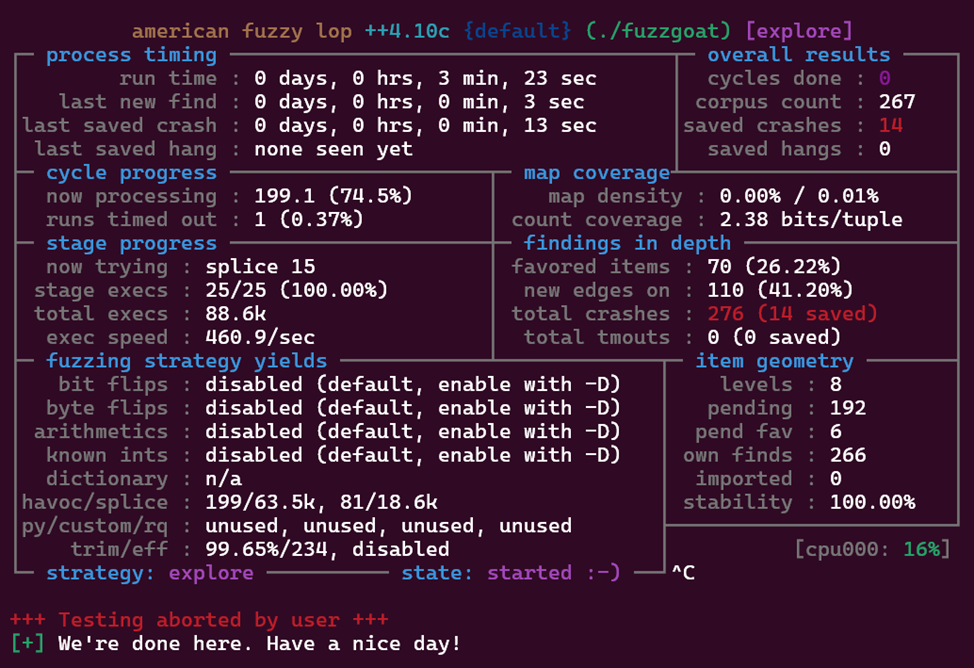
\includegraphics [scale=1] {my_folder/images/fuzz_panel}
	\caption{Панель мониторинга фаззинг-тестирования} 
	\label{fig:fuzz-panel-ch4}  
\end{figure}

На этой панели отображаются результаты процесса тестирования (\firef{fig:overall-res-ch4}).

\begin{figure}[ht] 
	\center
	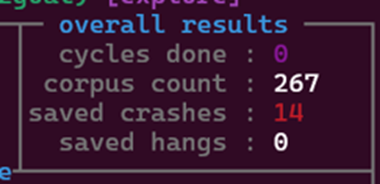
\includegraphics [scale=1] {my_folder/images/overall_res}
	\caption{Текущие результаты фаззинг-тестирования} 
	\label{fig:overall-res-ch4}  
\end{figure}

\begin{itemize}
	\item \textbf{cycles done:}??? Это количество полных циклов фаззинга, которое было выполнено. Один цикл обычно представляет собой полное исполнение всех тестов в корпусе данных (наборе уникальных тестовых случаев).
	\item \textbf{corpus count:} Количество уникальных тестов, которые в данный момент находятся в "корпусе" — наборе данных для тестирования. AFL++ использует этот корпус как исходный материал для генерации новых входных данных.
	\item \textbf{saved crashes:} Количество уникальных сбоев, которые были обнаружены.
	\item \textbf{saved hangs:} Количество случаев, когда тестируемая программа "зависала" или не отвечала в течение определенного времени, установленного AFL++.
\end{itemize}


\section{Анализ выявленных ошибок} \label{ch4:sec2}
В процессе фаззинга были обнаружены следующие ошибки (\firef{fig:errors-ch4}):

\begin{figure}[ht] 
	\center
	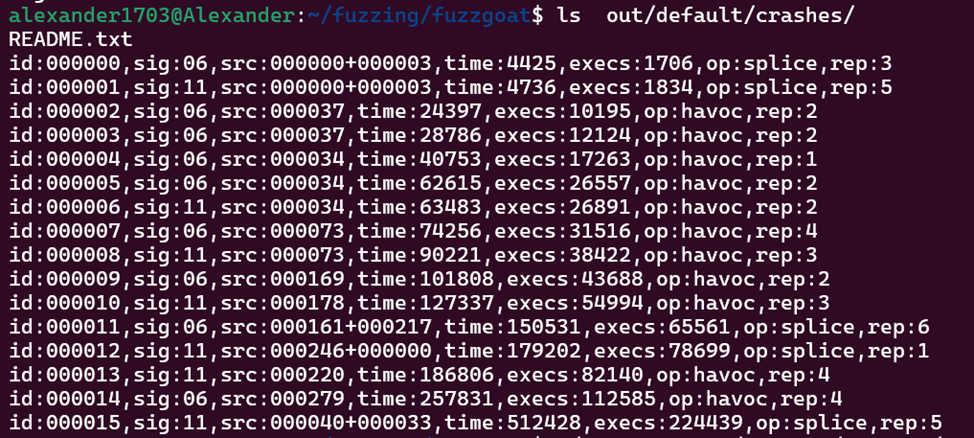
\includegraphics [scale=1] {my_folder/images/errors}
	\caption{Ошибки, выявленные в результате тестирования} 
	\label{fig:errors-ch4}  
\end{figure}

Рассмотрим как AFL именует файлы с ошибками:
id:000015,sig:11,src:000040+000033,time:512428,execs:224439,op:splice,rep:5.

\begin{itemize}
	\item \textbf{id:000015:}??? Это уникальный идентификатор ошибки.
	\item \textbf{sig:11:} Это номер сигнала, который был сгенерирован операционной системой при краше. Сигнал 11 в UNIX-подобных системах — это SIGSEGV, который означает нарушение доступа к памяти (segmentation fault).
	\item \textbf{src:000040+000033:} Это идентификаторы тестовых кейсов из корпуса, которые были использованы для генерации текущего входного файла. В данном случае файл был получен в результате "склеивания" (splice) двух входных файлов с идентификаторами 40 и 33.
	\item \textbf{time:512428:} Время в микросекундах, которое прошло с начала фаззинга до момента обнаружения данной ошибки.
	\item \textbf{execs:224439:} Количество выполнений (исполнений тестов), которое было произведено до обнаружения этой ошибки.
	\item \textbf{op:splice:} Операция, которая была применена к входному файлу, в данном случае "splice" означает, что AFL++ взял части из двух разных файлов корпуса и соединил их вместе, чтобы создать новый тестовый кейс.
	\item \textbf{rep:5:} Количество повторов (репликаций) данной операции, прежде чем был обнаружен краш. Это может означать, что ошибка возникла не с первого раза, а после нескольких попыток с различными мутациями.
\end{itemize}

Чтобы подробнее узнать о найденных ошибках нужно ввести команду
\begin{verbatim}
	./fuzzgoat out/default/crashes/id:000011,...,
\end{verbatim}
где:
\begin{itemize}
	\item ./fuzzgoat — исполняемый файл тестируемой программы
	\item out/default/crashes/id:000011,... - путь до файла
\end{itemize}

Рассмотрим некоторые из ошибок, которые были найдены (\firef{fig:errors-concrete-ch4}):
\begin{figure}[ht] 
	\center
	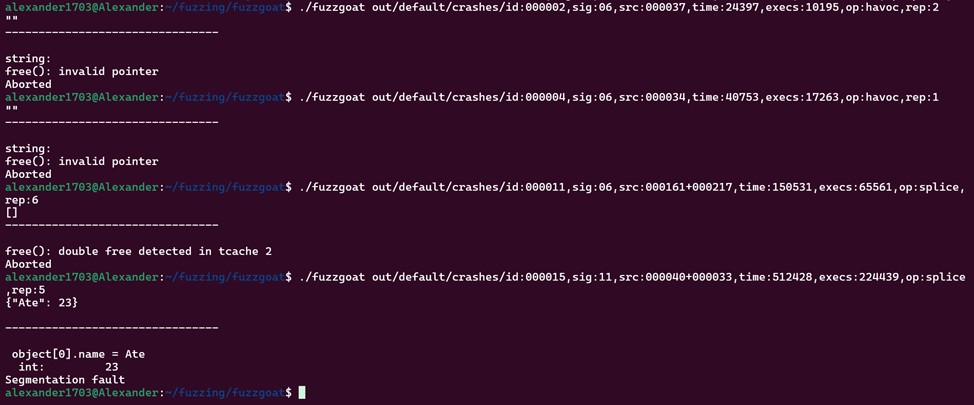
\includegraphics [scale=1] {my_folder/images/errors_concrete}
	\caption{Информация об ошибках, выявленных в процессе тестирования} 
	\label{fig:errors-concrete-ch4}  
\end{figure}

\textbf{free(): invalid pointer}

Попытка освободить память, которая не была выделена через malloc() или аналогичные функции, или уже была освобождена ранее. В данном случае, такая ошибка произошла дважды (id:000002 и id:000004):

\textbf{free(): double free detected in tcache 2}

Программа пытается освободить ту же область памяти более одного раза. 
Ошибка произошла при тесте с id:000011, что показывает, что определенные входные данные приводят к повторному освобождению уже освобожденной памяти.

\textbf{Segmentation fault}

Ошибка доступа к памяти вне выделенного сегмента. Обычно возникает, когда программа пытается читать или писать в память, к которой у нее нет доступа, или когда указатель на память не инициализирован.
Ошибка обнаружена при тестировании с id:000015.


К сожалению, точное место ошибки AFL не возвращает. AFL работает с уже скомпилированным кодом и не имеет прямого доступа к исходному коду программы, что делает невозможным указание точной строки или функции, где произошла ошибка. Фаззер отслеживает лишь факт возникновения сбоя, без анализа причин его возникновения на уровне исходного кода. Для определения конкретной причины и места сбоя необходимо использовать дополнительные инструменты, например профилировщики.

% не рекомендуется использовать отдельную section <<введение>> после лета 2020 года
%\section{Введение} \label{ch4:intro}

%Хорошим стилем является наличие введения к главе. Во введении может быть описана цель написания главы, а также приведена краткая структура главы. 
%	
%\section{Название параграфа} \label{ch4:sec1}
%
%\section{Название параграфа} \label{ch4:sec2}
%
%Пример ссылки на литературу \cite{avtonomova:fya,Peskov2004-ru,Kotelnikov2004-ru,Kotelnikov2004}.
%
%%\FloatBarrier % заставить рисунки и другие подвижные (float) элементы остановиться
%
%\section{Выводы} \label{ch4:conclusion}
%
%Текст выводов по главе \thechapter.

%% Вспомогательные команды - Additional commands
%
%\newpage % принудительное начало с новой страницы, использовать только в конце раздела
%\clearpage % осуществляется пакетом <<placeins>> в пределах секций
%\newpage\leavevmode\thispagestyle{empty}\newpage % 100 % начало новой страницы           	 % Глава 3
\ContinueChapterEnd % завершить размещение глав <<подряд>>
%% Завершение основной части

\chapter*{Заключение} \label{ch-conclusion}
\addcontentsline{toc}{chapter}{Заключение}	% в оглавление 

\textbf{ПОЛНОСТЬЮ дописываем (переписываем) с указанием также того, что сделал автор: рассмотрел различные виды фаззинга, изучил работу AFL++, развернул и на примере пофаззил, выявил, что не так все хорошо и далее общие слова (если Ваши...)}


Фаззинг, включая AFL++, является мощным инструментом для обнаружения уязвимостей в программном обеспечении с низкими затратами на внедрение и автоматизацией процесса тестирования. Этот метод позволяет обнаруживать широкий спектр ошибок. Благодаря автоматическому созданию и вводу большого количества случайных или псевдослучайных данных фаззинг позволяет проводить тестирование программного обеспечения быстро и эффективно.

Однако у фаззинга есть и ограничения. Во-первых, он имеет ограниченное покрытие кода, что может привести к пропуску некоторых ошибок, особенно если они находятся за пределами тестового покрытия. Во-вторых, некоторые типы ошибок, такие как логические ошибки, могут быть сложными для обнаружения с помощью фаззинга. Также важно отметить, что для достижения оптимальных результатов фаззинг требует дополнительной настройки, включая выбор правильных стратегий мутации и анализ результатов.

В целом, фаззинг, включая инструменты типа AFL++, является хорошим  дополнением к методам тестирования безопасности программного обеспечения. Он позволяет быстро обнаруживать уязвимости с низкими затратами на внедрение, что делает его привлекательным инструментом для разработчиков и исследователей. Однако для обеспечения полной безопасности программного обеспечения рекомендуется использовать фаззинг в сочетании с другими методами тестирования, такими как статический анализ кода и ручное тестирование.
        	 % Заключение

%% Наличие следующих перечней не исключает расшифровку сокращения и условного обозначения при первом упоминании в тексте!
%\chapter*{Список сокращений и условных обозначений}             % Заголовок
%\addcontentsline{toc}{chapter}{Список сокращений и условных обозначений}  % Добавляем его в оглавление
%\noindent
%\addtocounter{table}{-1}% Нужно откатить на единицу счетчик номеров таблиц, так как следующая таблица сделана для удобства представления информации по ГОСТ
%%\begin{longtabu} to \dimexpr \textwidth-5\tabcolsep {r X}
%\begin{longtabu} to \textwidth {r X} % Таблицу не прорисовываем!
%% Жирное начертание для математических символов может иметь
%% дополнительный смысл, поэтому они приводятся как в тексте
%% диссертации
%\textbf{DOI} & Digital Object Identifier. \\
%\textbf{WoS} & Web of Science. \\
%\textbf{ВКР}  & Выпускная квалификационная работа. \\
%\textbf{ТГ-объект}  & Текстово-графический объект. \\
%%$\begin{rcases}
%%a_n\\
%%b_n
%%\end{rcases}$  & 
%%\begin{minipage}{\linewidth}
%%Коэффициенты разложения Ми в дальнем поле, соответствующие
%%электрическим и магнитным мультиполям.
%%\end{minipage}
%%\\
%%${\boldsymbol{\hat{\mathrm e}}}$ & Единичный вектор. \\
%%$E_0$ & Амплитуда падающего поля.\\
%%$\begin{rcases}
%%a_n\\
%%b_n
%%\end{rcases}$  & 
%%Коэффициенты разложения Ми в дальнем поле соответствующие
%%электрическим и магнитным мультиполям ещё раз, но без окружения
%%minipage нет вертикального выравнивания по центру.
%%\\
%%$j$ & Тип функции Бесселя.\\
%%$k$ & Волновой вектор падающей волны.\\
%%
%%$\begin{rcases}
%%a_n\\
%%b_n
%%\end{rcases}$  & 
%%\begin{minipage}{\linewidth}
%%\vspace{0.7em}
%%Коэффициенты разложения Ми в дальнем поле соответствующие
%%электрическим и магнитным мультиполям, теперь окружение minipage есть
%%и добавленно много текста, так что описание группы условных
%%обозначений значительно превысило высоту этой группы... Для отбивки
%%пришлось добавить дополнительные отступы.
%%\vspace{0.5em}
%%\end{minipage}
%%\\
%%$L$ & Общее число слоёв.\\
%%$l$ & Номер слоя внутри стратифицированной сферы.\\
%%$\lambda$ & Длина волны электромагнитного излучения
%%в вакууме.\\
%%$n$ & Порядок мультиполя.\\
%%$\begin{rcases}
%%{\mathbf{N}}_{e1n}^{(j)}&{\mathbf{N}}_{o1n}^{(j)}\\
%%{\mathbf{M}_{o1n}^{(j)}}&{\mathbf{M}_{e1n}^{(j)}}
%%\end{rcases}$  & Сферические векторные гармоники.\\
%%$\mu$  & Магнитная проницаемость в вакууме.\\
%%$r,\theta,\phi$ & Полярные координаты.\\
%%$\omega$ & Частота падающей волны.\\
%%
%%  \textbf{BEM} & Boundary element method, метод граничных элементов.\\
%%  \textbf{CST MWS} & Computer Simulation Technology Microwave Studio.
%\end{longtabu}
		         % Необязательная рубрика! Список сокращений и условных обозначений

%\chapter*{Словарь терминов}             % Заголовок
%\addcontentsline{toc}{chapter}{Словарь терминов}  % Добавляем его в оглавление
%
%\textbf{TeX} --- язык вёрстки текста и издательская система, разработанные Дональдом Кнутом.
%
%\textbf{LaTeX} --- язык вёрстки текста и издательская система, разработанные Лэсли Лампортом как надстройка над TeX.
%
    		 % Необязательная рубрика! Словарь терминов
% По порядку после Списка сокращений и условных обозначений, если есть.	


%%% Не мянять - Do not modify
%%
%%
\clearpage                                  % В том числе гарантирует, что список литературы в оглавлении будет с правильным номером страницы
%\hypersetup{ urlcolor=black }               % Ссылки делаем чёрными
%\providecommand*{\BibDash}{}                % В стилях ugost2008 отключаем использование тире как разделителя 
\urlstyle{rm}                               % ссылки URL обычным шрифтом
\ifdefmacro{\microtypesetup}{\microtypesetup{protrusion=false}}{} % не рекомендуется применять пакет микротипографики к автоматически генерируемому списку литературы
%\newcommand{\fullbibtitle}{Список литературы} % (ГОСТ Р 7.0.11-2011, 4)
%\insertbibliofull  
%\noindent
%\begin{group}
\chapter*{Список использованных источников}	
\label{references}
\addcontentsline{toc}{chapter}{Список использованных источников}	% в оглавление 
\printbibliography[env=SSTfirst]                         % Подключаем Bib-базы
\begin{enumerate}[label=\arabic*.]
	\item Фаззинг-тестирование: QA Bible: \url{https://vladislaveremeev.gitbook.io/qa_bible/vidy-metody-urovni-testirovaniya/fazzing-testirovanie-fuzz-testing}
	
	\item Wikipedia: American Fuzzy Lop (software): \url{https://en.wikipedia.org/wiki/American_Fuzzy_Lop_(software)}
	
	\item Исследование инструментов фаззинга для
	генерации модульных тестов на Java - Александра Осипова:
	\url{https://dspace.spbu.ru/bitstream/11701/32418/1/Osipova_report.pdf}
	
	\item More about AFL - afl-1: \url{https://afl-1.readthedocs.io/en/latest/about_afl.html}
	
	\item Binary fuzzing strategies: what works, what doesn't - lcamtuf old blog: \url{https://lcamtuf.blogspot.com/2014/08/binary-fuzzing-strategies-what-works.html}
	\item Как провести фаззинг REST API с помощью RESTler - Habr: \url{https://habr.com/ru/companies/swordfish_security/articles/793514/l}
	
	\item Учебное пособие по фаззингу  - guru99: \url{https://www.guru99.com/ru/fuzz-testing.html}
	
	\item Обзор различных средств фаззинга как инструментов динамического анализа программного обеспечения. Мишечкин, М. В. - Молодой Ученый: \url{https://moluch.ru/archive/186/47575/}
	
	 	\item Фаззинг на пальцах. Часть 1: идея, техника и мера - Habr:
	 	 \url{https://habr.com/ru/companies/ussc/articles/771778/}
\end{enumerate}
%\ifdefmacro{\microtypesetup}{\microtypesetup{protrusion=true}}{}
%\urlstyle{tt}                               % возвращаем установки шрифта ссылок URL
%\hypersetup{ urlcolor={urlcolor} }          % Восстанавливаем цвет ссылок



%\urlstyle{rm}                               % ссылки URL обычным шрифтом
%\ifdefmacro{\microtypesetup}{\microtypesetup{protrusion=false}}{} % не рекомендуется применять пакет микротипографики к автоматически генерируемому списку литературы
%\insertbibliofull                           % Подключаем Bib-базы
%\ifdefmacro{\microtypesetup}{\microtypesetup{protrusion=true}}{}
%\urlstyle{tt}                               % возвращаем установки шрифта ссылок URL
		     % Список литературы

% Здесь можно поместить список иллюстративного материала

\appendix % не редактировать / keep unmodified


%\chapter{Краткие инструкции по настройке издательской системы \LaTeX}\label{appendix-MikTeX-TexStudio}							% Заголовок
%%\addcontentsline{toc}{chapter}{Second call for chapters to participate in the book Machine learning in analysis of biomedical and socio-economic data}	% Добавляем его в оглавление
%
%В SPbPU-BCI-template {\itshape автоматически выставляются необходимые настройки и в исходном тексте шаблона приведены примеры оформления текстово-графических объектов}, поэтому авторам достаточно заполнить имеющийся шаблон текстом главы (статьи), не вдаваясь в детали оформления, описанные далее. Возможный <<быстрый старт>> оформления главы (статьи) под Windows следующий\footnote{Внимание! Пример оформления подстрочной ссылки (сноски).}:
%
%\begin{enumerate}
%	\item Установка полной версии MikTeX  \cite{latex-miktex}.  В процессе установки лучше выставить параметр доустановки пакетов <<на лету>>.
%	
%	\item Установка TexStudio \cite{latex-texstudio}.
%	
%%		\item установка шрифтов PSCyr для работы с TimesNew\-Roman\-PSMT  	\href{https://github.com/AndreyAkinshin/Russian-Phd-LaTeX-Dissertation-Template/blob/master/PSCyr/Windows.md}{по данной инструкции}. В итоговом документе будет, скорее всего, использован Newton.
%	
%%	\item Переименование следующих файлов, где вместо \texttt{AuthorsSur\-names} необходимо подставить фамилии авторов (можно сокращать до первых четырех букв): 
%%	
%%	\begin{enumerate}
%%		\item Основной файл \texttt{Book\_title\_ch\_Authors\-Sur\-names.tex}.
%%		\item Библиография \texttt{biblio\textbackslash{}Book\_title\_bib\_Authors\-Sur\-na\-mes\-.bib}.
%%		\item Пользовательские настройки (при необходимости), \texttt{common\textbackslash{}Book\_\-tit\-le\_ext\_Authors\-Sur\-names.tex}. 
%%	\end{enumerate}
%%	
%%	\item После открытия основного файла \texttt{Book\_title\_ch\_Authors\-Sur\-names.tex} (с новым названием)   переименовать названия по аналогии в следующих командах \texttt{\textbackslash{}input\{\}}:
%%	
%%	\begin{enumerate}
%%		\item \texttt{biblio/Book\_title\_bib\_Authors\-Sur\-names.bib},
%%		\item \texttt{common/Book\_title\_ext\_Authors\-Sur\-names.tex (при необходимости) }.
%%	\end{enumerate}
%%	
%	
%	\item Запуск TexStudio и компиляция \verb|my_chapter.tex| с помощью команды <<Build\&View>> (например, с помощью двойной зелёной стрелки в верхней панели). {\itshape Иногда, для достижения нужного результата необходимо несколько раз скомпилировать документ.}
%	
%	\item В случае, если не отобразилась библиография, можно
%	
%	\begin{itemize}
%		\item воспользоваться командой Tools $\to$ Commands $\to$ Biber, затем запустив Build\&View;
%		
%		\item настроить автоматическое включение библиографии в настройках Options $\to$ Configure TexStudio $\to$ Build $\to$  Build\&View (оставить по умолчанию, если сборка происходит слишком долго): \texttt{txs:///pdflatex | txs:///biber | txs:///pdflatex | txs:///pdflatex | txs:///\-view-pdf}.
%	\end{itemize}
%	
%\end{enumerate}
%
%В случае возникновения ошибок, попробуйте скомпилировать документ до последних действий или внимательно ознакомьтесь с описанием проблемы в log-файле. Бывает полезным переход (по подсказке TexStudio) в нужную строку в pdf-файле или запрос с текстом ошибке в поисковиках. Наиболее вероятной проблемой при первой компиляции может быть отсутствие какого-либо установленного пакета \LaTeX. 
%
%В случае корректной работы настройки <<установка на лету>> все дополнительные пакеты будут скачиваться и устанавливаться в автоматическом режиме. Если доустановка пакетов осуществляется медленно (несколько пакетов за один запуск компилятора), то можно попробовать установить их в ручном режиме следующим образом:
%
%\begin{enumerate}[1.]
%	\item Запустите программу: меню $\to$ все программы $\to$ MikTeX $\to$ Maintenance (Admin) $\to$ MiKTeX Package Manager (Admin).
%	\item Пользуясь поиском, убедитесь, что нужный пакет присутствует, но не установлен (если пакет отсутствует воспользуйтесь сначала MiKTeX Update (Admin)).
%	\item Выделив строку с пакетом (возможно выбрать несколько или вообще все неустановленные пакеты), выполните установку Tools $\to$ Install или с помощью контекстного меню.
%	\item После завершения установки запустите программу MiKTeX Settings (Admin).
%	\item Обновите базу данных имен файлов Refresh FNDB.
%\end{enumerate}
%
%
%Для проверки текста статьи на русском языке полезно также воспользоваться настройками Options $\to$ Configure TexStudio $\to$ Language Checking $\to$  Default Language. Если русский язык <<ru\_RU>> не будет доступен в меню выбора, то необходимо вначале выполнить Import Dictionary, скачав из интернета любой русскоязычный словарь. 
%
%
%%\chapter{\normalfont\normalsize{}Часто задаваемые вопросы (FAQ)}\label{Appendix-FAQ}							% Заголовок
%%%\addcontentsline{toc}{chapter}{Second call for chapters to participate in the book Machine learning in analysis of biomedical and socio-economic data}	% Добавляем его в оглавление
%
%
%Далее приведены формулы \eqref{eq:Pi-app2}, \eqref{eq:Pi-app2-},  \firef{fig:spbpu_hydrotower-app2}, \firef{fig:spbpu_hydrotower-app2-}, \taref{tab:ToyCompare-app2}, \taref{tab:ToyCompare-app2-}.
%
%
%\begin{equation}% лучше не оставлять пропущенную строку (\par) перед окружениями для избежания лишних отсупов в pdf
%\label{eq:Pi-app2-} % eq - equations, далее название, ch поставлено для избежания дублирования
%\pi \approx 3,141.
%\end{equation}
%
%%
%\begin{figure}[ht!] 
%	\center
%	\includegraphics [scale=0.27] {my_folder/images//spbpu_hydrotower}
%	\caption{Вид на гидробашню СПбПУ \cite{spbpu-gallery}} 
%	\label{fig:spbpu_hydrotower-app2-}  
%\end{figure}
%
%\begin{table} [htbp]% Пример оформления таблицы
%	\centering\small
%	\caption{Представление данных для сквозного примера по ВКР \cite{Peskov2004}}%
%	\label{tab:ToyCompare-app2-}		
%	\begin{tabular}{|l|l|l|l|l|l|}
%		\hline
%		$G$&$m_1$&$m_2$&$m_3$&$m_4$&$K$\\
%		\hline
%		$g_1$&0&1&1&0&1\\ \hline
%		$g_2$&1&2&0&1&1\\ \hline
%		$g_3$&0&1&0&1&1\\ \hline
%		$g_4$&1&2&1&0&2\\ \hline
%		$g_5$&1&1&0&1&2\\ \hline
%		$g_6$&1&1&1&2&2\\ \hline		
%	\end{tabular}	
%	\normalsize% возвращаем шрифт к нормальному
%\end{table}
%
%
%
%
%\section{Параграф приложения}\label{app-2-1}							
%
%
%\subsection{Название подпараграфа} \label{ch2:subsec-title-abbr} %название по-русски
%
%
%Название подпараграфа оформляется с помощью команды  \texttt{\textbackslash{}subsection\{...\}}.
%
%Использование подподпараграфов в основной части крайне не рекомендуется.
%\subsubsection{Название подподпараграфа}\label{ch2:subsubsec-title-abbr} %название по-русски
%
%\begin{equation}% лучше не оставлять пропущенную строку (\par) перед окружениями для избежания лишних отсупов в pdf
%\label{eq:Pi-app2} % eq - equations, далее название, ch поставлено для избежания дублирования
%\pi \approx 3,141.
%\end{equation}
%%
%%
%\begin{figure}[ht!] 
%	\center
%	\includegraphics [scale=0.27] {my_folder/images//spbpu_hydrotower}
%	\caption{Вид на гидробашню СПбПУ \cite{spbpu-gallery}} 
%	\label{fig:spbpu_hydrotower-app2}  
%\end{figure}
%%
%
%
%
%
%\begin{table}[t!]% Пример оформления таблицы
%	\centering\small
%	\caption{Представление данных для сквозного примера по ВКР \cite{Peskov2004}}%
%	\label{tab:ToyCompare-app2}		
%	\begin{tabular}{|l|l|l|l|l|l|}
%		\hline
%		$G$&$m_1$&$m_2$&$m_3$&$m_4$&$K$\\
%		\hline
%		$g_1$&0&1&1&0&1\\ \hline
%		$g_2$&1&2&0&1&1\\ \hline
%		$g_3$&0&1&0&1&1\\ \hline
%		$g_4$&1&2&1&0&2\\ \hline
%		$g_5$&1&1&0&1&2\\ \hline
%		$g_6$&1&1&1&2&2\\ \hline		
%	\end{tabular}	
%	\normalsize% возвращаем шрифт к нормальному
%\end{table}
%
%
%%% В случае, когда таблица (рисунок) размещаются на последней странице, для переноса названия приложения на новую строку используем:
%\NewPage % начать новое приложение с новой страницы 			     % Приложение 1

%\chapter{Некоторые дополнительные примеры}\label{appendix-extra-examples}							% 
%
%В приложении\footnote{Внимание! Пример оформления подстрочной ссылки (сноски).} приведены формулы \eqref{eq:Pi-app}, \eqref{eq:Pi-app-}, \firef{fig:spbpu_hydrotower-app}, \firef{fig:spbpu_hydrotower-app-}, \taref{tab:ToyCompare-app}, \taref{tab:ToyCompare-app-}
%
%
%\begin{equation}% лучше не оставлять пропущенную строку (\par) перед окружениями для избежания лишних отсупов в pdf
%\label{eq:Pi-app-} % eq - equations, далее название, ch поставлено для избежания дублирования
%\pi \approx 3,141.
%\end{equation}
%%
%%
%\begin{figure}[ht!] 
%	\center
%	\includegraphics [scale=0.27] {my_folder/images//spbpu_hydrotower}
%	\caption{Вид на гидробашню СПбПУ \cite{spbpu-gallery}} 
%	\label{fig:spbpu_hydrotower-app-}  
%\end{figure}
%
%\begin{table} [htbp]% Пример оформления таблицы
%	\centering\small
%	\caption{Представление данных для сквозного примера по ВКР \cite{Peskov2004}}%
%	\label{tab:ToyCompare-app-}		
%	\begin{tabular}{|l|l|l|l|l|l|}
%		\hline
%		$G$&$m_1$&$m_2$&$m_3$&$m_4$&$K$\\
%		\hline
%		$g_1$&0&1&1&0&1\\ \hline
%		$g_2$&1&2&0&1&1\\ \hline
%		$g_3$&0&1&0&1&1\\ \hline
%		$g_4$&1&2&1&0&2\\ \hline
%		$g_5$&1&1&0&1&2\\ \hline
%		$g_6$&1&1&1&2&2\\ \hline		
%	\end{tabular}	
%	\normalsize% возвращаем шрифт к нормальному
%\end{table}
%
%
%
%
%\section{Подраздел приложения}\label{app-2-1}							
%
%
%\begin{equation}% лучше не оставлять пропущенную строку (\par) перед окружениями для избежания лишних отсупов в pdf
%\label{eq:Pi-app} % eq - equations, далее название, ch поставлено для избежания дублирования
%\pi \approx 3,141.
%\end{equation}
%%
%%
%\begin{figure}[ht!] 
%	\center
%	\includegraphics [scale=0.27] {my_folder/images//spbpu_hydrotower}
%	\caption{Вид на гидробашню СПбПУ \cite{spbpu-gallery}} 
%	\label{fig:spbpu_hydrotower-app}  
%\end{figure}
%
%\begin{table} [htbp]% Пример оформления таблицы
%	\centering\small
%	\caption{Представление данных для сквозного примера по ВКР \cite{Peskov2004}}%
%	\label{tab:ToyCompare-app}		
%	\begin{tabular}{|l|l|l|l|l|l|}
%		\hline
%		$G$&$m_1$&$m_2$&$m_3$&$m_4$&$K$\\
%		\hline
%		$g_1$&0&1&1&0&1\\ \hline
%		$g_2$&1&2&0&1&1\\ \hline
%		$g_3$&0&1&0&1&1\\ \hline
%		$g_4$&1&2&1&0&2\\ \hline
%		$g_5$&1&1&0&1&2\\ \hline
%		$g_6$&1&1&1&2&2\\ \hline		
%	\end{tabular}	
%	\normalsize% возвращаем шрифт к нормальному
%\end{table}
%
			 	 % Приложение 2


\end{document} % конец документа


%%% Удачной защиты ВКР! - Good luck on the thesis defense!
%%
%%% Поддержать проект
%%
%% Запросы на добавление / изменение просим писать на следующей странице:
%% https://github.com/ParkhomenkoV/SPbPU-student-thesis-template/issues
%%
%% Список пожеланий в файле шаблона <<TO-DO-list.tex>>
%%
%% Благодарности просим указывать в виде 
%%
%% 1. Добавление <<Звезды>> проекту https://github.com/ParkhomenkoV/SPbPU-student-thesis-template/stargazers
%%
%% 2. Добавления <<Сердечка>> и репоста проекта в социальных сетях:
%%		https://vk.com/latex_polytech 
%%		https://www.fb.com/groups/latex.polytech
%%

%%% Support project
%%
%% Requests on adding / modifications is better to be publishen on the following web-page:
%% https://github.com/ParkhomenkoV/SPbPU-student-thesis-template/issues
%%
%% Wishlist is in the template's file called <<TO-DO-list.tex>>
%%
%% Acknowledgements are better to be done in the form of 
%%
%% 1. Adding <<Star>> to the project https://github.com/ParkhomenkoV/SPbPU-student-t\dfrac{числит}{знамен}hesis-template/stargazers
%%
%% 2. Adding <<Likes>> and Project repost in the social networks:
%%		https://vk.com/latex_polytech 
%%		https://www.fb.com/groups/latex.polytech
%% 

% Check list при передаче ВКР:
% - Количество страниц в Задании 2. Если нет, то комментирование последней строки в my_task.tex
% - Зачистка всех вспомогательных файлов (Clear auxilary files) и компиляция ВКР не менее 3х раз